% Problem 16 - Start of Rotational Mechanical Control Systems
\begin{fold}
\newpage
% Problem 16 Start of Rotational Mechanical Control Systems

\newpage
\noindent\rule{\textwidth}{1pt}
\noindent\textbf{Problem 16} \hfill 
%palagay ulit dito 'yung problem statement
\\Solve for the Transfer Function, $\dfrac{\theta_1(s)}{T(s)}$, of the given Rotational Control System\\	
\begin{center}
	\begin{tikzpicture}[every node/.append style={font=\scriptsize}]
		% wall
		\def\brickw{0.24}   % brick width
		\def\brickh{0.18} % brick height
		\def\nrows{14}   % number of rows
		% draw bricks row by row
		\foreach \r in {0,...,\nrows} {
			% shift every other row
			\pgfmathparse{mod(\r,2)==0 ? 0 : 0.5*\brickw}
			\let\shift\pgfmathresult
			\foreach \c in {0,1} {
			\draw[thick] (\shift+\c*\brickw, \r*\brickh) rectangle ++(\brickw,\brickh);
		}}
		\draw (0,0) rectangle (0.6,2.7);
		% spring
		\draw (0.6,0.65) [cute inductor=] to (2,0.65);
		% mass damper
		\draw (0.6,1.4) to (0.8,1.4);
		\draw (0.8,1) to (0.8, 1.8);
		\draw (0.8,1) to (1.6, 1);
		\draw (0.8,1.8) to (1.6, 1.8);
		\draw (1.2, 1.2) to (1.2, 1.6);
		\draw (1.2,1.4) to (2, 1.4);
		%Inertia
  		\draw (2,1.8) -- (4.6,1.8);
  		\draw (2,0.3) -- (4.6,0.3);
  		\draw (2,1.05) ellipse (0.15 and 0.75);
  		\draw (4.6,0.3) arc[start angle=-90, end angle=90, x                radius=0.2, y radius=0.75];

		% spring
		\draw (4.8,0.65) [cute inductor=] to (6.2,0.65);
		% mass damper
		\draw (4.8,1.4) to (5,1.4);
		\draw (5,1) to (5, 1.8);
		\draw (5,1) to (5.8, 1);
		\draw (5,1.8) to (5.8, 1.8);
		\draw (5.4, 1.2) to (5.4, 1.6);
		\draw (5.4,1.4) to (6.2, 1.4);
		%Inertia
  		\draw (6.2,1.8) -- (8.8,1.8);
  		\draw (6.2,0.3) -- (8.8,0.3);
  		\draw (6.2,1.05) ellipse (0.15 and 0.75);
  		\draw (8.8,0.3) arc[start angle=-90, end angle=90, x                radius=0.2, y radius=0.75];

		% spring
		\draw (9,0.65) [cute inductor=] to (10.4,0.65);
		% mass damper
		\draw (9,1.4) to (9.2,1.4);
		\draw (9.2,1) to (9.2, 1.8);
		\draw (9.2,1) to (10, 1);
		\draw (9.2,1.8) to (10, 1.8);
		\draw (9.6, 1.2) to (9.6, 1.6);
		\draw (9.6,1.4) to (10.4, 1.4);
		%Inertia
  		\draw (10.4,1.8) -- (13,1.8);
  		\draw (10.4,0.3) -- (13,0.3);
  		\draw (10.4,1.05) ellipse (0.15 and 0.75);
  		\draw (13,0.3) arc[start angle=-90, end angle=90, x radius=0.2, y radius=0.75];

		% spring
		\draw (13.2,0.65) [cute inductor=] to (14.6,0.65);
		% mass damper
		\draw (13.2,1.4) to (13.4,1.4);
		\draw (13.4,1) to (13.4, 1.8);
		\draw (13.4,1) to (14.2, 1);
		\draw (13.4,1.8) to (14.2, 1.8);
		\draw (13.8, 1.2) to (13.8, 1.6);
		\draw (13.8,1.4) to (14.6, 1.4);
		% wall
		\def\brickw{0.24}   % brick width
		\def\brickh{0.18} % brick height
		\def\nrows{14}   % number of rows
		% draw bricks row by row
		\begin{scope}[shift={(14.6,0)}]
			\foreach \r in {0,...,\nrows} {
				% shift every other row
				\pgfmathparse{mod(\r,2)==0 ? 0 : 0.5*\brickw}
				\let\shift\pgfmathresult
				\foreach \c in {0,1} {
				\draw[thick] (\shift+\c*\brickw, \r*\brickh) rectangle ++(\brickw,\brickh);
			}}
			\draw (0,0) rectangle (0.6,2.7);
		\end{scope}
		
		% Label 1
		\node at (1.75, 2) {9 N-m-s/rad};
		\node at (1.75, 0) {2 N-m/rad};
		\node at (3.3, 1.05) {1 $kg-m^2$};
        % Label 2
		\node at (5.75, 2) {6 N-m-s/rad};
		\node at (5.75, 0) {5 N-m/rad};
		\node at (7.65, 1.05) {1 $kg-m^2$};
        % Label 3
		\node at (9.95, 2) {3 N-m-s/rad};
		\node at (9.95, 0) {2 N-m/rad};
		\node at (11.85, 1.05) {1 $kg-m^2$};
        % Label 4
		\node at (13.5, 2) {7 N-m-s/rad};
		\node at (13.75, 0) {4 N-m/rad};
		% Arrows 1
		\draw[<-,thick,cyan] (4.25,1.8) arc[start angle=45,end angle=315,x radius=0.5,y radius=1.1];
		\node[cyan] at (3.75,2.5) {$\theta_1(t)$};
		\draw[<-,thick,cyan] (3.5,1.8) arc[start angle=45,end angle=315,x radius=0.5,y radius=1.1];
		\node[cyan] at (3,2.5) {$T(t)$};
		% Arrows 2
		\draw[<-,thick, cyan] (8.25,1.8) arc[start angle=45,end angle=315,x radius=0.5,y radius=1];
		\node[cyan] at (8,2.5) {$\theta_2(t)$};
		% Arrows 3
		\draw[<-,thick,cyan] (12.25,1.8) arc[start angle=45,end angle=315,x radius=0.5,y radius=1];
		\node[cyan] at (12,2.5) {$\theta_3(t)$};
	\end{tikzpicture}
\end{center}
\noindent\rule{\textwidth}{1pt}

\noindent \textbf{\textit{Given:}}\\

\[
\begin{aligned}
J_1 &= 1\,\text{kg·m}^2 \qquad & f_{v1} &= 9\,\text{N·m·s/rad} \qquad & K_1 &= 2\,\text{N·m/rad} \\
J_2 &= 1\,\text{kg·m}^2 \qquad & f_{v2} &= 6\,\text{N·m·s/rad} \qquad & K_2 &= 5\,\text{N·m/rad} \\
J_3 &= 1\,\text{kg·m}^2 \qquad & f_{v3} &= 3\,\text{N·m·s/rad} \qquad & K_3 &= 2\,\text{N·m/rad} \\
&& f_{v4} &= 7\,\text{N·m·s/rad} \qquad & K_4 &= 4\,\text{N·m/rad}
\end{aligned}
\]


\noindent \textbf{\textit{Required:}}\\

\begin{center}
	$\dfrac{\theta_1(s)}{T(s)}$
\end{center}

\noindent \textbf{\textit{Solution:}}\\

	\begin{enumerate}[label=(\alph*),itemindent=*, itemindent=*, leftmargin=*, nolistsep]
		\item Transform the diagram to its Complex Domain.\\
		
\begin{center}
	\begin{tikzpicture}[every node/.append style={font=\scriptsize}]
		% wall
		\def\brickw{0.24}   % brick width
		\def\brickh{0.18} % brick height
		\def\nrows{14}   % number of rows
		% draw bricks row by row
		\foreach \r in {0,...,\nrows} {
			% shift every other row
			\pgfmathparse{mod(\r,2)==0 ? 0 : 0.5*\brickw}
			\let\shift\pgfmathresult
			\foreach \c in {0,1} {
			\draw[thick] (\shift+\c*\brickw, \r*\brickh) rectangle ++(\brickw,\brickh);
		}}
		\draw (0,0) rectangle (0.6,2.7);
		% spring
		\draw (0.6,0.65) [cute inductor=] to (2,0.65);
		% mass damper
		\draw (0.6,1.4) to (0.8,1.4);
		\draw (0.8,1) to (0.8, 1.8);
		\draw (0.8,1) to (1.6, 1);
		\draw (0.8,1.8) to (1.6, 1.8);
		\draw (1.2, 1.2) to (1.2, 1.6);
		\draw (1.2,1.4) to (2, 1.4);
		%Inertia
  		\draw (2,1.8) -- (4.6,1.8);
  		\draw (2,0.3) -- (4.6,0.3);
  		\draw (2,1.05) ellipse (0.15 and 0.75);
  		\draw (4.6,0.3) arc[start angle=-90, end angle=90, x                radius=0.2, y radius=0.75];

		% spring
		\draw (4.8,0.65) [cute inductor=] to (6.2,0.65);
		% mass damper
		\draw (4.8,1.4) to (5,1.4);
		\draw (5,1) to (5, 1.8);
		\draw (5,1) to (5.8, 1);
		\draw (5,1.8) to (5.8, 1.8);
		\draw (5.4, 1.2) to (5.4, 1.6);
		\draw (5.4,1.4) to (6.2, 1.4);
		%Inertia
  		\draw (6.2,1.8) -- (8.8,1.8);
  		\draw (6.2,0.3) -- (8.8,0.3);
  		\draw (6.2,1.05) ellipse (0.15 and 0.75);
  		\draw (8.8,0.3) arc[start angle=-90, end angle=90, x                radius=0.2, y radius=0.75];

		% spring
		\draw (9,0.65) [cute inductor=] to (10.4,0.65);
		% mass damper
		\draw (9,1.4) to (9.2,1.4);
		\draw (9.2,1) to (9.2, 1.8);
		\draw (9.2,1) to (10, 1);
		\draw (9.2,1.8) to (10, 1.8);
		\draw (9.6, 1.2) to (9.6, 1.6);
		\draw (9.6,1.4) to (10.4, 1.4);
		%Inertia
  		\draw (10.4,1.8) -- (13,1.8);
  		\draw (10.4,0.3) -- (13,0.3);
  		\draw (10.4,1.05) ellipse (0.15 and 0.75);
  		\draw (13,0.3) arc[start angle=-90, end angle=90, x                radius=0.2, y radius=0.75];

		% spring
		\draw (13.2,0.65) [cute inductor=] to (14.6,0.65);
		% mass damper
		\draw (13.2,1.4) to (13.4,1.4);
		\draw (13.4,1) to (13.4, 1.8);
		\draw (13.4,1) to (14.2, 1);
		\draw (13.4,1.8) to (14.2, 1.8);
		\draw (13.8, 1.2) to (13.8, 1.6);
		\draw (13.8,1.4) to (14.6, 1.4);
		% wall
		\def\brickw{0.24}   % brick width
		\def\brickh{0.18} % brick height
		\def\nrows{14}   % number of rows
		% draw bricks row by row
		\begin{scope}[shift={(14.6,0)}]
			\foreach \r in {0,...,\nrows} {
				% shift every other row
				\pgfmathparse{mod(\r,2)==0 ? 0 : 0.5*\brickw}
				\let\shift\pgfmathresult
				\foreach \c in {0,1} {
				\draw[thick] (\shift+\c*\brickw, \r*\brickh) rectangle ++(\brickw,\brickh);
			}}
			\draw (0,0) rectangle (0.6,2.7);
		\end{scope}
		
		% Label 1
		\node at (1.25, 2) {$9s$};
		\node at (1.25, 0) {$2$};
		\node at (3.3, 1.05) {$s^2$};
        % Label 2
		\node at (5.5, 2) {$6s$};
		\node at (5.5, 0) {$5$};
		\node at (7.65, 1.05) {$s^2$};
        % Label 3
		\node at (9.75, 2) {$3s$};
		\node at (9.75, 0) {$2$};
		\node at (11.85, 1.05) {$s^2$};
        % Label 4
		\node at (13.75, 2) {$7s$};
		\node at (13.9, 0) {$4$};
		% Arrows 1
		\draw[<-,thick,cyan] (4.25,1.8) arc[start angle=45,end angle=315,x radius=0.5,y radius=1.1];
		\node[cyan] at (3.75,2.5) {$\theta_1(s)$};
		\draw[<-,thick,cyan] (3.5,1.8) arc[start angle=45,end angle=315,x radius=0.5,y radius=1.1];
		\node[cyan] at (3,2.5) {$T(s)$};
		% Arrows 2
		\draw[<-,thick, cyan] (8.25,1.8) arc[start angle=45,end angle=315,x radius=0.5,y radius=1];
		\node[cyan] at (8,2.5) {$\theta_2(s)$};
		% Arrows 3
		\draw[<-,thick,cyan] (12.25,1.8) arc[start angle=45,end angle=315,x radius=0.5,y radius=1];
		\node[cyan] at (12,2.5) {$\theta_3(s)$};
	\end{tikzpicture}
\end{center}

\item Draw the Free Body Diagram of the Inertias\\[6pt]

        \begin{center}
                \centering
                \textbf{Free Body Diagram at $J_1$} \\[6pt]
				\vspace{15pt}
                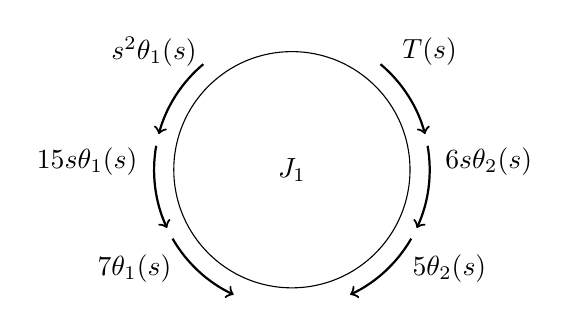
\begin{tikzpicture}
                    % Circle
                    \draw (0,0) circle (1.5);
                    \node at (0,0) {$J_1$};
                    % Left-hand Arrows
                    \draw[->, thick] (0,0) ++(130:1.75) arc[start angle=130, end angle=165, radius=1.75];
                    \node at (-1.75,1.5){$s^2\theta_1(s)$};
                    \draw[->, thick] (0,0) ++(170:1.75) arc[start angle=170, end angle=205, radius=1.75];
                    \node at (-2.6,0.1){$15s\theta_1(s)$};
                    \draw[->, thick] (0,0) ++(210:1.75) arc[start angle=210, end angle=245, radius=1.75];
                    \node at (-2,-1.25){$7\theta_1(s)$};
                    % Right-hand Arrows
                    \draw[->, thick] (0,0) ++(50:1.75) arc[start angle=50, end angle=15, radius=1.75];
                    \node at (1.75,1.5){$T(s)$};
                    \draw[->, thick] (0,0) ++(10:1.75) arc[start angle=10, end angle=-25, radius=1.75];
                    \node at (2.5,0.1){$6s\theta_2(s)$};
                    \draw[->, thick] (0,0) ++(-30:1.75) arc[start angle=-30, end angle=-65, radius=1.75];
                    \node at (2,-1.25){$5\theta_2(s)$};
                \end{tikzpicture}
        
                % Equations under J1
                \vspace{15pt}
        
                    $\sum T_0 = 0 \quad\text{(clockwise, +)}$ \\ \vspace{10pt}
                    $T(s) - (s^2+15s+7)\theta_1(s) + (6s+5)\theta_2(s) = 0$ \\ \vspace{10pt}
                    $T(s) = (s^2+15s+7)\theta_1(s) - (6s+5)\theta_2(s)$
        
		\end{center}
    \vspace{15pt}
        \begin{center}
            \centering
            %---------------- RIGHT SIDE: J2 ----------------%
                \textbf{Free Body Diagram at $J_2$} \\[6pt]
				\vspace{15pt}
                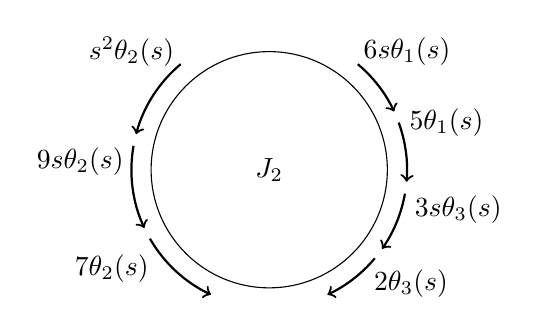
\begin{tikzpicture}
                    % Circle
                    \draw (0,0) circle (1.5);
                    \node at (0,0) {$J_2$};
                    % Left-hand Arrows
                    \draw[->, thick] (0,0) ++(130:1.75) arc[start angle=130, end angle=165, radius=1.75];
                    \node at (-1.75,1.5){$s^2\theta_2(s)$};
                    \draw[->, thick] (0,0) ++(170:1.75) arc[start angle=170, end angle=205, radius=1.75];
                    \node at (-2.4,0.1){$9s\theta_2(s)$};
                    \draw[->, thick] (0,0) ++(210:1.75) arc[start angle=210, end angle=245, radius=1.75];
                    \node at (-2,-1.25){$7\theta_2(s)$};
                    % Right-hand Arrows
                    \draw[->, thick] (0,0) ++(50:1.75) arc[start angle=50, end angle=25, radius=1.75];
                    \node at (1.75,1.5){$6s\theta_1(s)$};
                    \draw[->, thick] (0,0) ++(20:1.75) arc[start angle=20, end angle=-5, radius=1.75];
                    \node at (2.25,0.6){$5\theta_1(s)$};
                    \draw[->, thick] (0,0) ++(-10:1.75) arc[start angle=-10, end angle=-35, radius=1.75];
                    \node at (2.4,-0.5){$3s\theta_3(s)$};
                    \draw[->, thick] (0,0) ++(-40:1.75) arc[start angle=-40, end angle=-65, radius=1.75];
                    \node at (1.8,-1.45){$2\theta_3(s)$};
                \end{tikzpicture}
        
                % Equations under J2
        
        \vspace{15pt}

            $\sum T_0 = 0 \quad\text{(clockwise, +)}$ \\ \vspace{10pt}
            $0 = (6s+5)\theta_1(s) - (s^2+11s+16)\theta_2(s) + (3s+2)\theta_3(s)$\\ \vspace{10pt}
            $0 = -(6s+5)\theta_1(s) + (s^2+11s+16)\theta_2(s) - (3s+2)\theta_3(s)$

        
        \end{center}
    \vspace{15pt}
        \begin{center}
                \textbf{Free Body Diagram at $J_3$} \\[6pt]
				\vspace{15pt}
                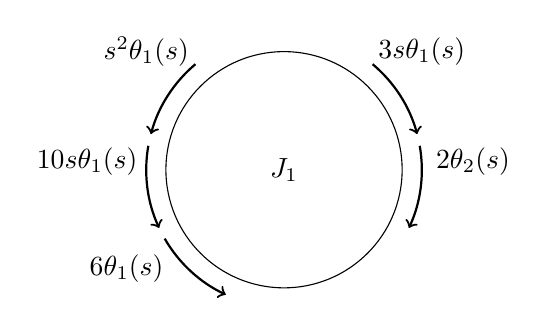
\begin{tikzpicture}
                    % Circle
                    \draw (0,0) circle (1.5);
                    \node at (0,0) {$J_1$};
                    % Left-hand Arrows
                    \draw[->, thick] (0,0) ++(130:1.75) arc[start angle=130, end angle=165, radius=1.75];
                    \node at (-1.75,1.5){$s^2\theta_1(s)$};
                    \draw[->, thick] (0,0) ++(170:1.75) arc[start angle=170, end angle=205, radius=1.75];
                    \node at (-2.5,0.1){$10s\theta_1(s)$};
                    \draw[->, thick] (0,0) ++(210:1.75) arc[start angle=210, end angle=245, radius=1.75];
                    \node at (-2,-1.25){$6\theta_1(s)$};
                    % Right-hand Arrows
                    \draw[->, thick] (0,0) ++(50:1.75) arc[start angle=50, end angle=15, radius=1.75];
                    \node at (1.75,1.5){$3s\theta_1(s)$};
                    \draw[->, thick] (0,0) ++(10:1.75) arc[start angle=10, end angle=-25, radius=1.75];
                    \node at (2.4,0.1){$2\theta_2(s)$};
                  
                \end{tikzpicture}
        
                % Equations under J3
                \vspace{15pt}
        

            $\sum T_0 = 0 \quad\text{(clockwise, +)}$ \\ \vspace{10pt}
            $0 = (3s+2)\theta_2(s) - (s^2 + 10s + 6)\theta_3(s)$ \\ \vspace{10pt}
            $0 = -(3s+2)\theta_2(s) + (s^2 + 10s + 6)\theta_3(s) $

            \end{center}
        
		\item Write the angular displacement equations and provide the matrix form
\begin{center}
	T(s) $= (s^2 + 15s + 7)\theta_1(s) - (6s + 5)\theta_2(s)$\\
	0 $= -(6s+5)\theta_1(s) + (s^2 + 9s + 7)\theta_2(s) - (3s + 2)\theta_3(s)$\\
	0 $= -(3s+2)\theta_2(s) + (s^2 + 10s + 6)\theta_3(s)$
	\[
		\begin{bmatrix}
		(s^2 + 15s + 7) & -(6s + 5) & 0\\
		-(6s + 5) & (s^2 + 9s + 7) & -(3s + 2)\\
		0 & -(3s + 2) & (s^2 + 10s + 6)
		\end{bmatrix}
		\begin{bmatrix}
		\theta_1(s) \\
		\theta_2(s) \\
		\theta_3(s)
		\end{bmatrix}
		=
		\begin{bmatrix}
		T(s)\\
		0\\
		0
		\end{bmatrix}
	\]\\
\end{center}
		\item Apply Cramer's Rule to get the value of the Transfer Function
\begin{center}
	\[
		\theta_1(s) = 
			\frac{\begin{vmatrix}
				T(s) & -(6s + 5) & 0\\
				0 & (s^2 + 9s + 7) & -(3s + 2)\\
				0 & -(3s + 2) & (s^2 + 10s + 6)
			\end{vmatrix}
		}{\begin{vmatrix}
				(s^2 + 15s + 7) & -(6s + 5) & 0\\
				-(6s + 5) & (s^2 + 9s + 7) & -(3s + 2)\\
				0 & -(3s + 2) & (s^2 + 10s + 6)
			\end{vmatrix}
		}
	\]
	\[
	\theta_1(s) = \frac{(s^4 + 19s^3 + 94s^2 + 112s + 38)T(s)}{s^6 + 34s^5 + 350s^4 + 1235s^3 + 1535s^2 + 744s + 116}
	\] 

	\[
	\boxed{\frac{\theta_1(s)}{T(s)} = \frac{s^4 + 19s^3 + 94s^2 + 112s + 38}{s^6 + 34s^5 + 350s^4 + 1235s^3 + 1535s^2 + 744s + 116}}
	\]
\end{center}
	\end{enumerate}

% End of Problem 16

\end{fold}

% Problem 17
\begin{fold}
\newpage
% Problem 

\newpage
\noindent\rule{\textwidth}{1pt}
\noindent\textbf{Problem 17} \hfill 
%palagay ulit dito 'yung problem statement
\\Solve for the Transfer Function, $\dfrac{\theta_1(s)}{T(s)}$, of the given Rotational Control system\\	
\begin{center}
	\begin{tikzpicture}[every node/.append style={font=\scriptsize}]
		% wall
		\def\brickw{0.24}   % brick width
		\def\brickh{0.18} % brick height
		\def\nrows{14}   % number of rows
		% draw bricks row by row
		\foreach \r in {0,...,\nrows} {
			% shift every other row
			\pgfmathparse{mod(\r,2)==0 ? 0 : 0.5*\brickw}
			\let\shift\pgfmathresult
			\foreach \c in {0,1} {
			\draw[thick] (\shift+\c*\brickw, \r*\brickh) rectangle ++(\brickw,\brickh);
		}}
		\draw (0,0) rectangle (0.6,2.7);
		% spring
		\draw (0.6,0.65) [cute inductor=] to (2,0.65);
		%Inertia
  		\draw (2,1.8) -- (4.6,1.8);
  		\draw (2,0.3) -- (4.6,0.3);
  		\draw (2,1.05) ellipse (0.15 and 0.75);
  		\draw (4.6,0.3) arc[start angle=-90, end angle=90, x                radius=0.2, y radius=0.75];

		% spring
		\draw (4.8,0.65) [cute inductor=] to (6.2,0.65);
		% mass damper
		\draw (4.8,1.4) to (5,1.4);
		\draw (5,1) to (5, 1.8);
		\draw (5,1) to (5.8, 1);
		\draw (5,1.8) to (5.8, 1.8);
		\draw (5.4, 1.2) to (5.4, 1.6);
		\draw (5.4,1.4) to (6.2, 1.4);
		%Inertia
  		\draw (6.2,1.8) -- (8.8,1.8);
  		\draw (6.2,0.3) -- (8.8,0.3);
  		\draw (6.2,1.05) ellipse (0.15 and 0.75);
  		\draw (8.8,0.3) arc[start angle=-90, end angle=90, x                radius=0.2, y radius=0.75];

		% spring
		\draw (9,0.65) [cute inductor=] to (10.4,0.65);
		% mass damper
		\draw (9,1.4) to (9.2,1.4);
		\draw (9.2,1) to (9.2, 1.8);
		\draw (9.2,1) to (10, 1);
		\draw (9.2,1.8) to (10, 1.8);
		\draw (9.6, 1.2) to (9.6, 1.6);
		\draw (9.6,1.4) to (10.4, 1.4);
		%Inertia
  		\draw (10.4,1.8) -- (13,1.8);
  		\draw (10.4,0.3) -- (13,0.3);
  		\draw (10.4,1.05) ellipse (0.15 and 0.75);
  		\draw (13,0.3) arc[start angle=-90, end angle=90, x                radius=0.2, y radius=0.75];

		% spring
		\draw (13.2,0.65) [cute inductor=] to (14.6,0.65);
		% wall
		\def\brickw{0.24}   % brick width
		\def\brickh{0.18} % brick height
		\def\nrows{14}   % number of rows
		% draw bricks row by row
		\begin{scope}[shift={(14.6,0)}]
			\foreach \r in {0,...,\nrows} {
				% shift every other row
				\pgfmathparse{mod(\r,2)==0 ? 0 : 0.5*\brickw}
				\let\shift\pgfmathresult
				\foreach \c in {0,1} {
				\draw[thick] (\shift+\c*\brickw, \r*\brickh) rectangle ++(\brickw,\brickh);
			}}
			\draw (0,0) rectangle (0.6,2.7);
		\end{scope}
		
		% Label 1
		\node at (1.75, 0) {$15N-m/rad$};
		\node at (3.3, 1.05) {$4kg-m^2$};
        % Label 2
		\node at (5.5, 2) {$8N-m-s/rad$};
		\node at (5.5, 0) {$16N-m/rad$};
		\node at (7.65, 1.05) {$19kg-m^2$};
        % Label 3
		\node at (9.75, 2) {$9N-m-s/rad$};
		\node at (9.75, 0) {$12N-m/rad$};
		\node at (11.85, 1.05) {$7kg-m^s$};
        % Label 4
		\node at (13.5, 0) {$15N-m/rad$};
		% Arrows 1
		\draw[<-,thick,cyan] (4.25,1.8) arc[start angle=45,end angle=315,x radius=0.5,y radius=1.1];
		\node[cyan] at (3.75,2.5) {$\theta_1(t)$};
		\draw[<-,thick,cyan] (3.5,1.8) arc[start angle=45,end angle=315,x radius=0.5,y radius=1.1];
		\node[cyan] at (2.85,2.5) {$T(t)$};
		% Arrows 2
		\draw[<-,thick, cyan] (8.25,1.8) arc[start angle=45,end angle=315,x radius=0.5,y radius=1];
		\node[cyan] at (8,2.5) {$\theta_2(t)$};
		% Arrows 3
		\draw[<-,thick,cyan] (12.25,1.8) arc[start angle=45,end angle=315,x radius=0.5,y radius=1];
		\node[cyan] at (12,2.5) {$\theta_3(t)$};
	\end{tikzpicture}
\end{center}
\noindent\rule{\textwidth}{1pt}

\noindent \textbf{\textit{Given:}}\\

\[
\begin{aligned}
J_1 &= 4\,\text{kg·m}^2 & f_{v1} &= 8\,\text{N·m·s/rad} & K_1 &= 15\,\text{N·m/rad} \\
J_2 &= 19\,\text{kg·m}^2 & f_{v2} &= 9\,\text{N·m·s/rad} & K_2 &= 16\,\text{N·m/rad} \\
J_3 &= 7\,\text{kg·m}^2 & & & K_3 &= 12\,\text{N·m/rad} \\
& & & & K_4 &= 15\,\text{N·m/rad}
\end{aligned}
\]



\noindent \textbf{\textit{Required:}}\\

\begin{center}
    $\dfrac{\theta_1(s)}{T(s)}$
\end{center}


\noindent \textbf{\textit{Solution:}}\\

	\begin{enumerate}[label=(\alph*),itemindent=*, itemindent=*, leftmargin=*, nolistsep]
		\item Transform the diagram to its Complex Domain.\\
		
\begin{center}
	\begin{tikzpicture}[every node/.append style={font=\scriptsize}]
		% wall
		\def\brickw{0.24}   % brick width
		\def\brickh{0.18} % brick height
		\def\nrows{14}   % number of rows
		% draw bricks row by row
		\foreach \r in {0,...,\nrows} {
			% shift every other row
			\pgfmathparse{mod(\r,2)==0 ? 0 : 0.5*\brickw}
			\let\shift\pgfmathresult
			\foreach \c in {0,1} {
			\draw[thick] (\shift+\c*\brickw, \r*\brickh) rectangle ++(\brickw,\brickh);
		}}
		\draw (0,0) rectangle (0.6,2.7);
		% spring
		\draw (0.6,0.65) [cute inductor=] to (2,0.65);
		%Inertia
  		\draw (2,1.8) -- (4.6,1.8);
  		\draw (2,0.3) -- (4.6,0.3);
  		\draw (2,1.05) ellipse (0.15 and 0.75);
  		\draw (4.6,0.3) arc[start angle=-90, end angle=90, x                radius=0.2, y radius=0.75];

		% spring
		\draw (4.8,0.65) [cute inductor=] to (6.2,0.65);
		% mass damper
		\draw (4.8,1.4) to (5,1.4);
		\draw (5,1) to (5, 1.8);
		\draw (5,1) to (5.8, 1);
		\draw (5,1.8) to (5.8, 1.8);
		\draw (5.4, 1.2) to (5.4, 1.6);
		\draw (5.4,1.4) to (6.2, 1.4);
		%Inertia
  		\draw (6.2,1.8) -- (8.8,1.8);
  		\draw (6.2,0.3) -- (8.8,0.3);
  		\draw (6.2,1.05) ellipse (0.15 and 0.75);
  		\draw (8.8,0.3) arc[start angle=-90, end angle=90, x                radius=0.2, y radius=0.75];

		% spring
		\draw (9,0.65) [cute inductor=] to (10.4,0.65);
		% mass damper
		\draw (9,1.4) to (9.2,1.4);
		\draw (9.2,1) to (9.2, 1.8);
		\draw (9.2,1) to (10, 1);
		\draw (9.2,1.8) to (10, 1.8);
		\draw (9.6, 1.2) to (9.6, 1.6);
		\draw (9.6,1.4) to (10.4, 1.4);
		%Inertia
  		\draw (10.4,1.8) -- (13,1.8);
  		\draw (10.4,0.3) -- (13,0.3);
  		\draw (10.4,1.05) ellipse (0.15 and 0.75);
  		\draw (13,0.3) arc[start angle=-90, end angle=90, x                radius=0.2, y radius=0.75];

		% spring
		\draw (13.2,0.65) [cute inductor=] to (14.6,0.65);
		% wall
		\def\brickw{0.24}   % brick width
		\def\brickh{0.18} % brick height
		\def\nrows{14}   % number of rows
		% draw bricks row by row
		\begin{scope}[shift={(14.6,0)}]
			\foreach \r in {0,...,\nrows} {
				% shift every other row
				\pgfmathparse{mod(\r,2)==0 ? 0 : 0.5*\brickw}
				\let\shift\pgfmathresult
				\foreach \c in {0,1} {
				\draw[thick] (\shift+\c*\brickw, \r*\brickh) rectangle ++(\brickw,\brickh);
			}}
			\draw (0,0) rectangle (0.6,2.7);
		\end{scope}
		
		% Label 1
		\node at (1.25, 0) {$15$};
		\node at (3.3, 1.05) {$4s^2$};
        % Label 2
		\node at (5.5, 2) {$8s$};
		\node at (5.5, 0) {$16$};
		\node at (7.65, 1.05) {$19s^2$};
        % Label 3
		\node at (9.75, 2) {$9s$};
		\node at (9.75, 0) {$12$};
		\node at (11.85, 1.05) {$7s^2$};
        % Label 4
		\node at (13.9, 0) {$15$};
		% Arrows 1
		\draw[<-,thick,cyan] (4.25,1.8) arc[start angle=45,end angle=315,x radius=0.5,y radius=1.1];
		\node[cyan] at (3.75,2.5) {$\theta_1(s)$};
		\draw[<-,thick,cyan] (3.5,1.8) arc[start angle=45,end angle=315,x radius=0.5,y radius=1.1];
		\node[cyan] at (3,2.5) {$T(s)$};
		% Arrows 2
		\draw[<-,thick, cyan] (8,1.8) arc[start angle=45,end angle=315,x radius=0.5,y radius=1];
		\node[cyan] at (7.25,2.5) {$\theta_2(s)$};
		% Arrows 3
		\draw[<-,thick,cyan] (12,1.8) arc[start angle=45,end angle=315,x radius=0.5,y radius=1];
		\node[cyan] at (11.5,2.5) {$\theta_3(s)$};
	\end{tikzpicture}
\end{center}

\item Draw the Free Body Diagram of the Inertias\\[6pt]

        \begin{center}
                \textbf{Free Body Diagram at $J_1$} \\[6pt]
				\vspace{15pt}
                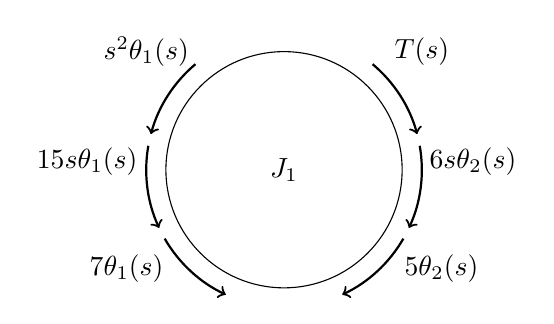
\begin{tikzpicture}
                    % Circle
                    \draw (0,0) circle (1.5);
                    \node at (0,0) {$J_1$};
                    % Left-hand Arrows
                    \draw[->, thick] (0,0) ++(130:1.75) arc[start angle=130, end angle=165, radius=1.75];
                    \node at (-1.75,1.5){$s^2\theta_1(s)$};
                    \draw[->, thick] (0,0) ++(170:1.75) arc[start angle=170, end angle=205, radius=1.75];
                    \node at (-2.5,0.1){$15s\theta_1(s)$};
                    \draw[->, thick] (0,0) ++(210:1.75) arc[start angle=210, end angle=245, radius=1.75];
                    \node at (-2,-1.25){$7\theta_1(s)$};
                    % Right-hand Arrows
                    \draw[->, thick] (0,0) ++(50:1.75) arc[start angle=50, end angle=15, radius=1.75];
                    \node at (1.75,1.5){$T(s)$};
                    \draw[->, thick] (0,0) ++(10:1.75) arc[start angle=10, end angle=-25, radius=1.75];
                    \node at (2.4,0.1){$6s\theta_2(s)$};
                    \draw[->, thick] (0,0) ++(-30:1.75) arc[start angle=-30, end angle=-65, radius=1.75];
                    \node at (2,-1.25){$5\theta_2(s)$};
                \end{tikzpicture}
        
                % Equations under J1
                \vspace{15pt}
        
                $\sum T_0 = 0 \quad\text{(clockwise, +)}$ \\ \vspace{10pt}
                $T(s) - (4s^2+8s+3)\theta_1(s) + (8s+16)\theta_2(s)  = 0$ \\ \vspace{10pt}
                $T(s) = (4s^2+8s+3)\theta_1(s)  - (8s+16)\theta_2(s)$ 

		\end{center}
    \vspace{15pt}
        \begin{center}
                \textbf{Free Body Diagram at $J_2$} \\[6pt]
				\vspace{15pt}
                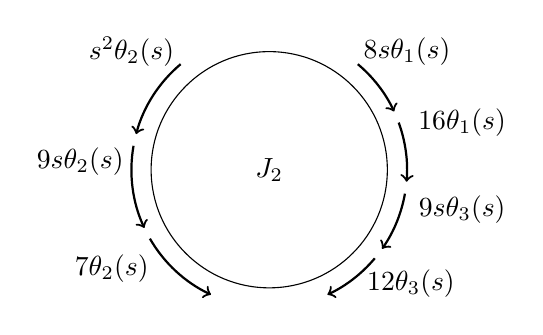
\begin{tikzpicture}
                    % Circle
                    \draw (0,0) circle (1.5);
                    \node at (0,0) {$J_2$};
                    % Left-hand Arrows
                    \draw[->, thick] (0,0) ++(130:1.75) arc[start angle=130, end angle=165, radius=1.75];
                    \node at (-1.75,1.5){$s^2\theta_2(s)$};
                    \draw[->, thick] (0,0) ++(170:1.75) arc[start angle=170, end angle=205, radius=1.75];
                    \node at (-2.4,0.1){$9s\theta_2(s)$};
                    \draw[->, thick] (0,0) ++(210:1.75) arc[start angle=210, end angle=245, radius=1.75];
                    \node at (-2,-1.25){$7\theta_2(s)$};
                    % Right-hand Arrows
                    \draw[->, thick] (0,0) ++(50:1.75) arc[start angle=50, end angle=25, radius=1.75];
                    \node at (1.75,1.5){$8s\theta_1(s)$};
                    \draw[->, thick] (0,0) ++(20:1.75) arc[start angle=20, end angle=-5, radius=1.75];
                    \node at (2.45,0.6){$16\theta_1(s)$};
                    \draw[->, thick] (0,0) ++(-10:1.75) arc[start angle=-10, end angle=-35, radius=1.75];
                    \node at (2.45,-0.5){$9s\theta_3(s)$};
                    \draw[->, thick] (0,0) ++(-40:1.75) arc[start angle=-40, end angle=-65, radius=1.75];
                    \node at (1.8,-1.45){$12\theta_3(s)$};
                \end{tikzpicture}
        
                % Equations under J2
        
        \vspace{15pt}
        

            $\sum T_0 = 0 \quad\text{(clockwise, +)} $\\ \vspace{10pt}
            $0 = (8s+16)\theta_1(s)  - (19s^2+17s+28)\theta_2(s)  + (9s+12)\theta_3(s)$ \\ \vspace{10pt}
            $0 = (-8s+16)\theta_1(s)  + (19s^2+17s+28)\theta_2(s)  - (9s+12)\theta_3(s)$ 

        \end{center}
        \vspace{15pt}
        \begin{center}
                \textbf{Free Body Diagram at $J_3$} \\[6pt]
				\vspace{15pt}
                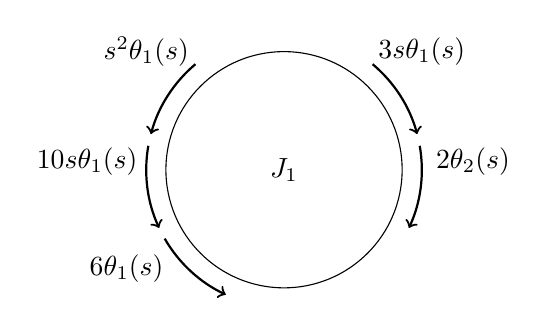
\begin{tikzpicture}
                    % Circle
                    \draw (0,0) circle (1.5);
                    \node at (0,0) {$J_1$};
                    % Left-hand Arrows
                    \draw[->, thick] (0,0) ++(130:1.75) arc[start angle=130, end angle=165, radius=1.75];
                    \node at (-1.75,1.5){$s^2\theta_1(s)$};
                    \draw[->, thick] (0,0) ++(170:1.75) arc[start angle=170, end angle=205, radius=1.75];
                    \node at (-2.5,0.1){$10s\theta_1(s)$};
                    \draw[->, thick] (0,0) ++(210:1.75) arc[start angle=210, end angle=245, radius=1.75];
                    \node at (-2,-1.25){$6\theta_1(s)$};
                    % Right-hand Arrows
                    \draw[->, thick] (0,0) ++(50:1.75) arc[start angle=50, end angle=15, radius=1.75];
                    \node at (1.75,1.5){$3s\theta_1(s)$};
                    \draw[->, thick] (0,0) ++(10:1.75) arc[start angle=10, end angle=-25, radius=1.75];
                    \node at (2.4,0.1){$2\theta_2(s)$};
                  
                \end{tikzpicture}
        
                % Equations under J1
                \vspace{15pt}
        

            $\sum T_0 = 0 \quad\text{(clockwise, +)}$ \\ \vspace{10pt}
            $0 = (9s+12)\theta_2(s)  - (7s^2 + 9s + 27)\theta_3(s)$  \\ \vspace{10pt}
            $0 = -(9s+12)\theta_2(s)  + (7s^2 + 9s + 27)\theta_3(s)$ 


        \end{center}

        \vspace{15pt}

		\item Write the angular displacement equations and provide the matrix form
\begin{center}
	T(s) $= (4s^2 + 8s + 3)\theta_1(s) - (8s + 16)\theta_2(s)$\\
	0 $= -(8s + 16)\theta_1(s) + (19s^2 + 17s + 28)\theta_2(s) - (9s + 12)\theta_3(s)$\\
	0 $= -(9s + 12)\theta_2(s) + (7s^2 + 9s + 27)\theta_3(s)$
	\[
		\begin{bmatrix}
		(4s^2 + 8s + 3) & -(8s + 16) & 0\\
		-(8s + 16) & (19s^2 + 17s + 28) & -(9s + 12)\\
		0 & -(9s + 12) & (7s^2 + 9s + 27)
		\end{bmatrix}
		\begin{bmatrix}
		\theta_1(s) \\
		\theta_2(s) \\
		\theta_3(s)
		\end{bmatrix}
		=
		\begin{bmatrix}
		T(s)\\
		0\\
		0
		\end{bmatrix}
	\]\\
\end{center}
		\item Apply Cramer's Rule to get the value of the Transfer Function
\begin{center}
	\[
		\theta_1(s) = 
			\frac{\begin{vmatrix}
				T(s) & -(8s + 16) & 0\\
				0 & (19s^2 + 17s + 28) & -(9s + 12)\\
				0 & -(9s + 12) & (7s^2 + 9s + 27)
			\end{vmatrix}
		}{\begin{vmatrix}
				(4s^2 + 8s + 3) & -(8s + 16) & 0\\
				-(8s + 16) & (19s^2 + 17s + 28) & -(9s + 12)\\
				0 & -(9s + 12) & (7s^2 + 9s + 27)
			\end{vmatrix}
		}
	\]
	\[
	\theta_1(s) = \frac{(133s^4 + 290s^3 + 781s^2 + 495s + 612)T(s)}{1862s^6 + 5124s^5 + 16929s^4 + 19800s^3 + 30915s^2 + 11025s + 12060}
	\] 

	\[
	\boxed{\frac{\theta_1(s)}{T(s)} = \frac{133s^4 + 290s^3 + 781s^2 + 495s + 612}{1862s^6 + 5124s^5 + 16929s^4 + 19800s^3 + 30915s^2 + 11025s + 12060}}
	\]
\end{center}
	\end{enumerate}

% End of Problem 17

\end{fold}

% Problem 18
\begin{fold}
\newpage
% Problem 18
\noindent\rule{\textwidth}{1pt}

\noindent\textbf{Problem 18} \hfill 
%palagay ulit dito 'yung problem statement
\\Solve for the Transfer Function, $\dfrac{\theta_1(s)}{T(s)}$, of the given Rotational Control System\\	
\begin{center}
	\begin{tikzpicture}[every node/.append style={font=\scriptsize}]
		% wall
            
		\def\brickw{0.24}   % brick width
		\def\brickh{0.18} % brick height
		\def\nrows{22}   % number of rows
		% draw bricks row by row
        \begin{scope}[shift={(-2,0)}]
		\foreach \r in {0,...,\nrows} {
			% shift every other row
			\pgfmathparse{mod(\r,2)==0 ? 0 : 0.5*\brickw}
			\let\shift\pgfmathresult
			\foreach \c in {0,1} {
			\draw[thick] (\shift+\c*\brickw, \r*\brickh) rectangle ++(\brickw,\brickh);
		}}
		\draw (0,0) rectangle (0.6,4.14);
        
            \end{scope}
		% spring
		\draw (-1.4,0.65) [cute inductor=] to (1.5,0.65);
		% mass damper
		\draw (-1.4,1.4) to (-0.2,1.4);
            \begin{scope}[shift={(-1,0)}]
		\draw (0.8,1) to (0.8, 1.8);
		\draw (0.8,1) to (1.6, 1);
		\draw (0.8,1.8) to (1.6, 1.8);
		\draw (1.2, 1.2) to (1.2, 1.6);
            \end{scope}
		\draw (0.2,1.4) to (1.5, 1.4);
		%Inertia
  		\draw (1.5,1.8) -- (4.1,1.8);
  		\draw (1.5,0.3) -- (4.1,0.3);
  		\draw (1.5,1.05) ellipse (0.15 and 0.75);
  		\draw (4.1,0.3) arc[start angle=-90, end angle=90, x                radius=0.2, y radius=0.75];

		% spring
		\draw (4.3,0.65) [cute inductor=] to (6.2,0.65);
		% mass damper
		\draw (4.3,1.4) to (4.75,1.4);
            \begin{scope}[shift={(-0.25,0)}]
		\draw (5,1) to (5, 1.8);
		\draw (5,1) to (5.8, 1);
		\draw (5,1.8) to (5.8, 1.8);
		\draw (5.4, 1.2) to (5.4, 1.6);
            \end{scope}
		\draw (5.15,1.4) to (6.2, 1.4);
		%Inertia
  		\draw (6.2,4.5) -- (8.8,4.5);
  		\draw (6.2,0) -- (8.8,0);
  		\draw (6.2,2.25) ellipse (0.2 and 2.25);
  		\draw (8.8,0) arc[start angle=-90, end angle=90, x                radius=0.275, y radius=2.25];
            % long damper and spring
            \draw (-1.4,3) [cute inductor=] to (6.2,3);
		% mass damper
		\draw (-1.4,3.75) to (2.05,3.75);
            \begin{scope}[shift={(-1,0)}]
		\draw (3.05,3.35) to (3.05, 4.15);
		\draw (3.05,3.35) to (3.85, 3.35);
		\draw (3.05,4.15) to (3.85, 4.15);
		\draw (3.45, 3.55) to (3.45, 3.95);
            \end{scope}
		\draw (2.45,3.75) to (6.2, 3.75);

		% spring
		\draw (9.05,1.65) [cute inductor=] to (12.4,1.65);
		% mass damper
		\draw (9.05,2.4) to (10.2,2.4);
            \begin{scope}[shift={(1,0)}]
		\draw (9.2,2) to (9.2, 2.8);
		\draw (9.2,2) to (10, 2);
		\draw (9.2,2.8) to (10, 2.8);
		\draw (9.6, 2.2) to (9.6, 2.6);
            \end{scope}
		\draw (10.6,2.4) to (12.4, 2.4);
		% wall
		\def\brickw{0.24}   % brick width
		\def\brickh{0.18} % brick height
		\def\nrows{22}   % number of rows
		% draw bricks row by row
		\begin{scope}[shift={(12.4,0)}]
			\foreach \r in {0,...,\nrows} {
				% shift every other row
				\pgfmathparse{mod(\r,2)==0 ? 0 : 0.5*\brickw}
				\let\shift\pgfmathresult
				\foreach \c in {0,1} {
				\draw[thick] (\shift+\c*\brickw, \r*\brickh) rectangle ++(\brickw,\brickh);
			}}
			\draw (0,0) rectangle (0.6,4.14);
		\end{scope}
		
		\node[scale=0.75] at (0.2, 2) {$1N-m-s/rad$};
		\node[scale=0.75] at (0.2, 0) {$1N-m/rad$};
		\node[scale=0.75] at (2.8, 1.05) {$1kg-m^2$};
        % Label 2
		\node[scale=0.75] at (4.65, 2) {$1N-m-s/rad$};
		\node[scale=0.75] at (4.75, 0) {$1N-m/rad$};
		\node[scale=0.75] at (7.65, 2.25) {$1kg-m^2$};
            \node[scale=0.75] at (2.75, 4.5) {$1N-m-s/rad$};
            \node[scale=0.75] at (2.65, 2.5) {$1N-m/rad$};
        % Label 3
		\node[scale=0.75] at (10.5, 3) {$1 N-m-s/rad$};
		\node[scale=0.75] at (10.5, 1.25) {$1 N-m/rad$};

		% Arrows 1
		\draw[<-,cyan] (3.75,1.8) arc[start angle=45,end angle=315,x radius=0.5,y radius=1.1];
		\node[cyan] at (3.5,-0.3) {$\theta_1(t)$};
		\draw[<-,cyan] (3,1.8) arc[start angle=45,end angle=315,x radius=0.5,y radius=1.1];
		\node[cyan] at (2.75,-0.3) {$T(t)$};
		% Arrows 2
		\draw[<-, cyan] (8.25,4.7) arc[start angle=60,end angle=300,x radius=0.5,y radius=2.8];
		\node[cyan] at (8.05,5.35) {$\theta_2(t)$};
	\end{tikzpicture}
\end{center}

\noindent\rule{\textwidth}{1pt}

\noindent \textbf{\textit{Given:}}\\

\[
\begin{aligned}
J_1 &= 1\,\text{kg·m}^2 \qquad & f_{v1} &= 1\,\text{N·m·s/rad} \qquad & K_1 &= 1\,\text{N·m/rad} \\
J_2 &= 1\,\text{kg·m}^2 \qquad & f_{v2} &= 1\,\text{N·m·s/rad} \qquad & K_2 &= 1\,\text{N·m/rad} \\
&& f_{v3} &= 1\,\text{N·m·s/rad} \qquad & K_3 &= 1\,\text{N·m/rad} \\
&& f_{v4} &= 1\,\text{N·m·s/rad} \qquad & K_4 &= 1\,\text{N·m/rad}
\end{aligned}
\]


\noindent \textbf{\textit{Required:}}\\

\begin{center}
	 $\dfrac{\theta_1(s)}{T(s)}$
\end{center}

	\noindent \textbf{\textit{Solution:}}\\

		\begin{enumerate}[label=(\alph*),itemindent=*, itemindent=*, leftmargin=*, nolistsep]
		\item Draw the Free Body Diagram of the Inertias\\[6pt]
\vspace{20pt}
			\begin{center}
					\textbf{Free Body Diagram at $J_1$} \\[6pt]
					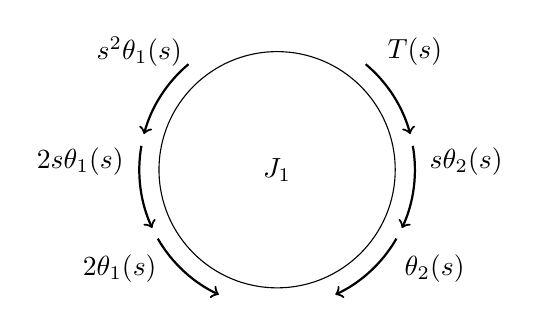
\begin{tikzpicture}
						% Circle
						\draw (0,0) circle (1.5);
						\node at (0,0) {$J_1$};
						% Left-hand Arrows
						\draw[->, thick] (0,0) ++(130:1.75) arc[start angle=130, end angle=165, radius=1.75];
						\node at (-1.75,1.5){$s^2\theta_1(s)$};
						\draw[->, thick] (0,0) ++(170:1.75) arc[start angle=170, end angle=205, radius=1.75];
						\node at (-2.5,0.1){$2s\theta_1(s)$};
						\draw[->, thick] (0,0) ++(210:1.75) arc[start angle=210, end angle=245, radius=1.75];
						\node at (-2,-1.25){$2\theta_1(s)$};
						% Right-hand Arrows
						\draw[->, thick] (0,0) ++(50:1.75) arc[start angle=50, end angle=15, radius=1.75];
						\node at (1.75,1.5){$T(s)$};
						\draw[->, thick] (0,0) ++(10:1.75) arc[start angle=10, end angle=-25, radius=1.75];
						\node at (2.4,0.1){$s\theta_2(s)$};
						\draw[->, thick] (0,0) ++(-30:1.75) arc[start angle=-30, end angle=-65, radius=1.75];
						\node at (2,-1.25){$\theta_2(s)$};
					\end{tikzpicture}
			
					% Equations under J1
					\vspace{25pt}
			
				$\sum T_0 = 0 \quad\text{(clockwise, +)}$ \\ \vspace{10pt}
				$0 = T(s) - (s^2 + 2s + 2)\theta_1(s) + (s+1)\theta_2(s)$\\ \vspace{10pt}
				$T(s) = (s^2 + 2s + 2)\theta_1(s) - (s+1)\theta_2(s)$
\newpage
				\end{center}
				\vspace{10pt}
				%---------------- RIGHT SIDE: J2 ----------------%
				\begin{center}
					\textbf{Free Body Diagram at $J_2$} \\[6pt]
					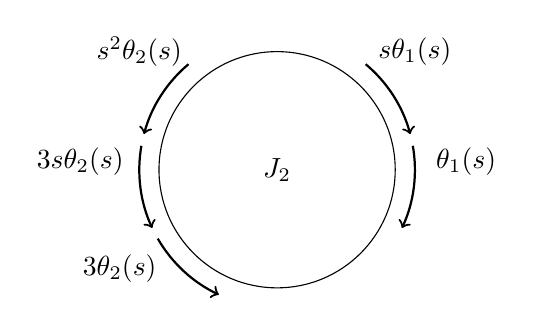
\begin{tikzpicture}
						% Circle
						\draw (0,0) circle (1.5);
						\node at (0,0) {$J_2$};
						% Left-hand Arrows
						\draw[->, thick] (0,0) ++(130:1.75) arc[start angle=130, end angle=165, radius=1.75];
						\node at (-1.75,1.5){$s^2\theta_2(s)$};
						\draw[->, thick] (0,0) ++(170:1.75) arc[start angle=170, end angle=205, radius=1.75];
						\node at (-2.5,0.1){$3s\theta_2(s)$};
						\draw[->, thick] (0,0) ++(210:1.75) arc[start angle=210, end angle=245, radius=1.75];
						\node at (-2,-1.25){$3\theta_2(s)$};
						% Right-hand Arrows
						\draw[->, thick] (0,0) ++(50:1.75) arc[start angle=50, end angle=15, radius=1.75];
						\node at (1.75,1.5){$s\theta_1(s)$};
						\draw[->, thick] (0,0) ++(10:1.75) arc[start angle=10, end angle=-25, radius=1.75];
						\node at (2.4,0.1){$\theta_1(s)$};
					\end{tikzpicture}
			
					% Equations under J2
			
			\vspace{15pt}
			
			$\sum T_0 = 0 \quad\text{(clockwise, +)}$ \\ \vspace{10pt}
			$0 = (s+1)\theta_1(s) - (s^2 + 3s + 3)\theta_2(s)$\\ \vspace{10pt}
			$0 = -(s+1)\theta_1 + (s^2 + 3s + 3)\theta_2$

			\end{center}
			\vspace{15pt}

			\item Write the angular displacement equations and provide the matrix form
	\begin{center}
		T(s) $= (s^2 + 2s + 2)\theta_1(s) - (s+1)\theta_2(s)$\\
		0 $= -(s+1)\theta_1(s) + (s^2 + 3s + 3)\theta_2(s)$
		\[
			\begin{bmatrix}
			(s^2 + 2s + 2) & -(s+1)\\
			-(s+1) & (s^2 + 3s + 3)
			\end{bmatrix}
			\begin{bmatrix}
			\theta_1(s) \\
			\theta_2(s)
			\end{bmatrix}
			=
			\begin{bmatrix}
			T(s)\\
			0
			\end{bmatrix}
		\]\\
	\end{center}
			\item Apply Cramer's Rule to get the value of the Transfer Function
	\begin{center}
		\[
			\theta_1(s) = 
				\frac{\begin{vmatrix}
					T(s) & -(s+1)\\
					0 & (s^2 + 3s + 3)
				\end{vmatrix}
			}{\begin{vmatrix}
					(s^2 + 2s + 2) & -(s+1)\\
					-(s+1) & (s^2 + 3s + 3)
				\end{vmatrix}
			}
		\]
		\[
		\theta_1(s) = \frac{(s^2 + 3s + 3)T(s)}{s^4 + 5s^3 + 10s^2 + 10s + 5}
		\] 

		\[
		\boxed{\frac{\theta_1(s)}{T(s)} = \frac{s^2 + 3s + 3}{s^4 + 5s^3 + 10s^2 + 10s + 5}}
		\]
	\end{center}

\end{enumerate}

\end{fold}

% Problem 19
\begin{fold}
\newpage

\newpage
\noindent\rule{\textwidth}{1pt}
\noindent\textbf{Problem 19} \hfill 
%palagay ulit dito 'yung problem statement
\\Solve for the Transfer Function, $\dfrac{\theta_1(s)}{T(s)}$, of the given Rotational Control system\\	
\begin{center}
	\begin{tikzpicture}[every node/.append style={font=\scriptsize}]
		% wall
            
		\def\brickw{0.24}   % brick width
		\def\brickh{0.18} % brick height
		\def\nrows{22}   % number of rows
		% draw bricks row by row
        \begin{scope}[shift={(-2,0)}]
		\foreach \r in {0,...,\nrows} {
			% shift every other row
			\pgfmathparse{mod(\r,2)==0 ? 0 : 0.5*\brickw}
			\let\shift\pgfmathresult
			\foreach \c in {0,1} {
			\draw[thick] (\shift+\c*\brickw, \r*\brickh) rectangle ++(\brickw,\brickh);
		}}
		\draw (0,0) rectangle (0.6,4.14);
        
            \end{scope}
		% spring
		\draw (-1.4,1.1) [cute inductor=] to (1.5,1.1);
		%Inertia
  		\draw (1.5,1.8) -- (4.1,1.8);
  		\draw (1.5,0.3) -- (4.1,0.3);
  		\draw (1.5,1.05) ellipse (0.15 and 0.75);
  		\draw (4.1,0.3) arc[start angle=-90, end angle=90, x                radius=0.2, y radius=0.75];

		% spring
		\draw (4.3,0.65) [cute inductor=] to (6.2,0.65);
		% mass damper
		\draw (4.3,1.4) to (4.75,1.4);
            \begin{scope}[shift={(-0.25,0)}]
		\draw (5,1) to (5, 1.8);
		\draw (5,1) to (5.8, 1);
		\draw (5,1.8) to (5.8, 1.8);
		\draw (5.4, 1.2) to (5.4, 1.6);
            \end{scope}
		\draw (5.15,1.4) to (6.2, 1.4);
		%Inertia
  		\draw (6.2,4.5) -- (8.8,4.5);
  		\draw (6.2,0) -- (8.8,0);
  		\draw (6.2,2.25) ellipse (0.2 and 2.25);
  		\draw (8.8,0) arc[start angle=-90, end angle=90, x                radius=0.275, y radius=2.25];
            % long damper and spring
            \draw (-1.4,3.5) [cute inductor=] to (6.2,3.5);
		% spring
		\draw (9.05,1.65) [cute inductor=] to (12.4,1.65);
		% mass damper
		\draw (9.05,2.4) to (10.2,2.4);
            \begin{scope}[shift={(1,0)}]
		\draw (9.2,2) to (9.2, 2.8);
		\draw (9.2,2) to (10, 2);
		\draw (9.2,2.8) to (10, 2.8);
		\draw (9.6, 2.2) to (9.6, 2.6);
            \end{scope}
		\draw (10.6,2.4) to (12.4, 2.4);
		% wall
		\def\brickw{0.24}   % brick width
		\def\brickh{0.18} % brick height
		\def\nrows{22}   % number of rows
		% draw bricks row by row
		\begin{scope}[shift={(12.4,0)}]
			\foreach \r in {0,...,\nrows} {
				% shift every other row
				\pgfmathparse{mod(\r,2)==0 ? 0 : 0.5*\brickw}
				\let\shift\pgfmathresult
				\foreach \c in {0,1} {
				\draw[thick] (\shift+\c*\brickw, \r*\brickh) rectangle ++(\brickw,\brickh);
			}}
			\draw (0,0) rectangle (0.6,4.14);
		\end{scope}
		
	% Label 1
		\node[scale=0.75] at (0.1, 1.5) {$9N-m/rad$};
		\node[scale=0.75] at (2.8, 1.05) {$8kg-m^2$};
        % Label 2
		\node[scale=0.75] at (4.65, 2) {$2N-m-s/rad$};
		\node[scale=0.75] at (4.75, 0) {$3N-m/rad$};
		\node[scale=0.75] at (7.65, 2.25) {$1kg-m^2$};
            \node[scale=0.75] at (2.35, 4) {$6N-m/rad$};
        % Label 3
		\node[scale=0.75] at (10.5, 3) {$9 N-m-s/rad$};
		\node[scale=0.75] at (10.5, 1.25) {$7 N-m/rad$};

		% Arrows 1
		\draw[<-,cyan] (3.75,1.8) arc[start angle=45,end angle=315,x radius=0.5,y radius=1.1];
		\node[cyan] at (3.5,-0.3) {$\theta_1(t)$};
		\draw[<-,cyan] (3,1.8) arc[start angle=45,end angle=315,x radius=0.5,y radius=1.1];
		\node[cyan] at (2.75,-0.3) {$T(t)$};
		% Arrows 2
		\draw[<-, cyan] (8.25,4.7) arc[start angle=60,end angle=300,x radius=0.5,y radius=2.8];
		\node[cyan] at (8.05,5.35) {$\theta_2(t)$};
	\end{tikzpicture}
\end{center}

\noindent\rule{\textwidth}{1pt}

\noindent \textbf{\textit{Given:}}\\

\[
\begin{aligned}
J_1 &= 1\,\text{kg·m}^2 \qquad & f_{v1} &= 2\,\text{N·m·s/rad} \qquad & K_1 &= 9\,\text{N·m/rad} \\
J_2 &= 1\,\text{kg·m}^2 \qquad & f_{v2} &= 9\,\text{N·m·s/rad} \qquad & K_2 &= 3\,\text{N·m/rad} \\
&&& & K_3 &= 7\,\text{N·m/rad} \\
&&& & K_4 &= 6\,\text{N·m/rad}
\end{aligned}
\]

\noindent \textbf{\textit{Required:}}\\

\begin{center}
	$\dfrac{\theta_1(s)}{T(s)}$
\end{center}

\noindent \textbf{\textit{Solution:}}\\

	\begin{enumerate}[label=(\alph*),itemindent=*, itemindent=*, leftmargin=*, nolistsep]
		\item Draw the Free Body Diagram of the Inertias\\[6pt]

        \begin{center}
                \textbf{Free Body Diagram at $J_1$} \\[6pt]
                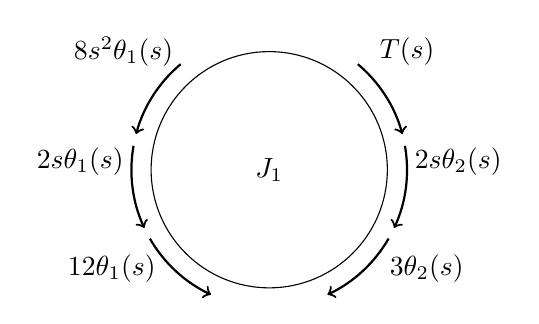
\begin{tikzpicture}
                    % Circle
                    \draw (0,0) circle (1.5);
                    \node at (0,0) {$J_1$};
                    % Left-hand Arrows
                    \draw[->, thick] (0,0) ++(130:1.75) arc[start angle=130, end angle=165, radius=1.75];
                    \node at (-1.85,1.5){$8s^2\theta_1(s)$};
                    \draw[->, thick] (0,0) ++(170:1.75) arc[start angle=170, end angle=205, radius=1.75];
                    \node at (-2.4,0.1){$2s\theta_1(s)$};
                    \draw[->, thick] (0,0) ++(210:1.75) arc[start angle=210, end angle=245, radius=1.75];
                    \node at (-2,-1.25){$12\theta_1(s)$};
                    % Right-hand Arrows
                    \draw[->, thick] (0,0) ++(50:1.75) arc[start angle=50, end angle=15, radius=1.75];
                    \node at (1.75,1.5){$T(s)$};
                    \draw[->, thick] (0,0) ++(10:1.75) arc[start angle=10, end angle=-25, radius=1.75];
                    \node at (2.4,0.1){$2s\theta_2(s)$};
                    \draw[->, thick] (0,0) ++(-30:1.75) arc[start angle=-30, end angle=-65, radius=1.75];
                    \node at (2,-1.25){$3\theta_2(s)$};
                \end{tikzpicture}
        
                % Equations under J1
                \vspace{15pt}
            	$\sum T_0 = 0 \quad\text{(clockwise, +)}$ \\ \vspace{10pt} 
            	$T(s) - (8s^2+2s+12)\theta_1 + (2s+3)\theta_2 = 0$ \\ \vspace{10pt} 
            	$T(s) = (8s^2+2s+12)\theta_1 - (2s+3)\theta_2$

            \end{center}
\newpage			
			\vspace{15pt} 
            %---------------- RIGHT SIDE: J2 ----------------%
            \begin{center}
                \textbf{Free Body Diagram at $J_2$} \\[6pt]
                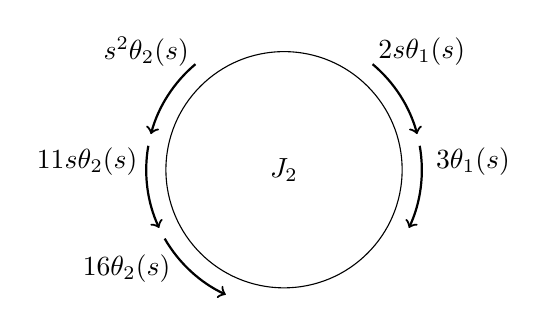
\begin{tikzpicture}
                    % Circle
                    \draw (0,0) circle (1.5);
                    \node at (0,0) {$J_2$};
                    % Left-hand Arrows
                    \draw[->, thick] (0,0) ++(130:1.75) arc[start angle=130, end angle=165, radius=1.75];
                    \node at (-1.75,1.5){$s^2\theta_2(s)$};
                    \draw[->, thick] (0,0) ++(170:1.75) arc[start angle=170, end angle=205, radius=1.75];
                    \node at (-2.5,0.1){$11s\theta_2(s)$};
                    \draw[->, thick] (0,0) ++(210:1.75) arc[start angle=210, end angle=245, radius=1.75];
                    \node at (-2,-1.25){$16\theta_2(s)$};
                    % Right-hand Arrows
                    \draw[->, thick] (0,0) ++(50:1.75) arc[start angle=50, end angle=15, radius=1.75];
                    \node at (1.75,1.5){$2s\theta_1(s)$};
                    \draw[->, thick] (0,0) ++(10:1.75) arc[start angle=10, end angle=-25, radius=1.75];
                    \node at (2.4,0.1){$3\theta_1(s)$};
                \end{tikzpicture}
        
                % Equations under J2
        
        \vspace{15pt}
        
            $\sum T_0 = 0 \quad\text{(clockwise, +)}$ \\ \vspace{10pt} 
            $0 = (2s+3)\theta_1 - (s^2+11s+16)\theta_2$ \\ \vspace{10pt} 
            $0 = -(2s+3)\theta_1 + (s^2+11s+16)\theta_2$

        
        \end{center}

        \vspace{15pt}

		\item Write the angular displacement equations and provide the matrix form
\begin{center}
	$T(s) = (8s^2+2s+12)\theta_1(s) - (2s+3)\theta_2(s)$\\
	$0 = -(2s+1)\theta_1(s) + (s^2+11s+16)\theta_2(s)$\\
	\[
		\begin{bmatrix}
		(8s^2+2s+12) & -(2s+3)\\
		-(2s+3) & (s^2+11s+16)\\
		\end{bmatrix}
		\begin{bmatrix}
		\theta_1(s) \\
		\theta_2(s)
		\end{bmatrix}
		=
		\begin{bmatrix}
		T(s)\\
		0\\
		\end{bmatrix}
	\]\\
\end{center}
		\item Apply Cramer's Rule to get the value of the Transfer Function
\begin{center}
	\[
		\theta_1(s) = 
			\frac{\begin{vmatrix}
				T(s) & -(2s+3)\\
		          0 & (s^2+11s+16)\\
			\end{vmatrix}
		}{\begin{vmatrix}
				(8s^2+2s+12) & -(2s+3)\\
		          -(2s+3) & (s^2+11s+16)\\
			\end{vmatrix}
		}
	\]
	\[
	\theta_1(s) = \frac{(s^2 + 11s + 16)T(s)}{8s^4 + 90s^3 + 158s^2 + 152s + 183}
	\] 

	\[
	\boxed{\frac{\theta_1(s)}{T(s)} = \frac{(s^2 + 11s + 16)}{8s^4 + 90s^3 + 158s^2 + 152s + 183}}
	\]
\end{center}
	\end{enumerate}
\end{fold}

% Problem 20
\begin{fold}
\newpage
% Problem 20

\newpage
\noindent\rule{\textwidth}{1pt}
\noindent\textbf{Problem 20} \hfill 
%palagay ulit dito 'yung problem statement
\\Solve for the Transfer Function, $\dfrac{\theta_1(s)}{T(s)}$, of the given Rotational Control System\\	
\begin{center}
	\begin{tikzpicture}[every node/.append style={font=\scriptsize}]
		% wall
            
		\def\brickw{0.24}   % brick width
		\def\brickh{0.18} % brick height
		\def\nrows{22}   % number of rows
		% draw bricks row by row
        \begin{scope}[shift={(-2,0)}]
		\foreach \r in {0,...,\nrows} {
			% shift every other row
			\pgfmathparse{mod(\r,2)==0 ? 0 : 0.5*\brickw}
			\let\shift\pgfmathresult
			\foreach \c in {0,1} {
			\draw[thick] (\shift+\c*\brickw, \r*\brickh) rectangle ++(\brickw,\brickh);
		}}
		\draw (0,0) rectangle (0.6,4.14);
        
            \end{scope}
		% spring
		\draw (-1.4,0.65) [cute inductor=] to (1.5,0.65);
		% mass damper
		\draw (-1.4,1.4) to (-0.2,1.4);
            \begin{scope}[shift={(-1,0)}]
		\draw (0.8,1) to (0.8, 1.8);
		\draw (0.8,1) to (1.6, 1);
		\draw (0.8,1.8) to (1.6, 1.8);
		\draw (1.2, 1.2) to (1.2, 1.6);
            \end{scope}
		\draw (0.2,1.4) to (1.5, 1.4);
		%Inertia
  		\draw (1.5,1.8) -- (4.1,1.8);
  		\draw (1.5,0.3) -- (4.1,0.3);
  		\draw (1.5,1.05) ellipse (0.15 and 0.75);
  		\draw (4.1,0.3) arc[start angle=-90, end angle=90, x                radius=0.2, y radius=0.75];

        \begin{scope}[shift={(0,2.5)}]
            % spring
    		\draw (-1.4,0.65) [cute inductor=] to (1.5,0.65);
    		% mass damper
    		\draw (-1.4,1.4) to (-0.2,1.4);
                \begin{scope}[shift={(-1,0)}]
    		\draw (0.8,1) to (0.8, 1.8);
    		\draw (0.8,1) to (1.6, 1);
    		\draw (0.8,1.8) to (1.6, 1.8);
    		\draw (1.2, 1.2) to (1.2, 1.6);
                \end{scope}
    		\draw (0.2,1.4) to (1.5, 1.4);
    		%Inertia
      		\draw (1.5,1.8) -- (4.1,1.8);
      		\draw (1.5,0.3) -- (4.1,0.3);
      		\draw (1.5,1.05) ellipse (0.15 and 0.75);
      		\draw (4.1,0.3) arc[start angle=-90, end angle=90, x                radius=0.2, y radius=0.75];
        % spring
		\draw (4.3,0.65) [cute inductor=] to (6.2,0.65);
		% mass damper
		\draw (4.3,1.4) to (4.75,1.4);
            \begin{scope}[shift={(-0.25,0)}]
		\draw (5,1) to (5, 1.8);
		\draw (5,1) to (5.8, 1);
		\draw (5,1.8) to (5.8, 1.8);
		\draw (5.4, 1.2) to (5.4, 1.6);
            \end{scope}
		\draw (5.15,1.4) to (6.2, 1.4);
        \end{scope}
        
		% spring
		\draw (4.3,0.65) [cute inductor=] to (6.2,0.65);
		% mass damper
		\draw (4.3,1.4) to (4.75,1.4);
            \begin{scope}[shift={(-0.25,0)}]
		\draw (5,1) to (5, 1.8);
		\draw (5,1) to (5.8, 1);
		\draw (5,1.8) to (5.8, 1.8);
		\draw (5.4, 1.2) to (5.4, 1.6);
            \end{scope}
		\draw (5.15,1.4) to (6.2, 1.4);
		%Inertia
  		\draw (6.2,4.5) -- (8.8,4.5);
  		\draw (6.2,0) -- (8.8,0);
  		\draw (6.2,2.25) ellipse (0.2 and 2.25);
  		\draw (8.8,0) arc[start angle=-90, end angle=90, x                radius=0.275, y radius=2.25];

		% spring
		\draw (9.05,1.65) [cute inductor=] to (12.4,1.65);
		% mass damper
		\draw (9.05,2.4) to (10.2,2.4);
            \begin{scope}[shift={(1,0)}]
		\draw (9.2,2) to (9.2, 2.8);
		\draw (9.2,2) to (10, 2);
		\draw (9.2,2.8) to (10, 2.8);
		\draw (9.6, 2.2) to (9.6, 2.6);
            \end{scope}
		\draw (10.6,2.4) to (12.4, 2.4);
		% wall
		\def\brickw{0.24}   % brick width
		\def\brickh{0.18} % brick height
		\def\nrows{22}   % number of rows
		% draw bricks row by row
		\begin{scope}[shift={(12.4,0)}]
			\foreach \r in {0,...,\nrows} {
				% shift every other row
				\pgfmathparse{mod(\r,2)==0 ? 0 : 0.5*\brickw}
				\let\shift\pgfmathresult
				\foreach \c in {0,1} {
				\draw[thick] (\shift+\c*\brickw, \r*\brickh) rectangle ++(\brickw,\brickh);
			}}
			\draw (0,0) rectangle (0.6,4.14);
		\end{scope}
		
	    % Label 1
		\node[scale=0.75] at (0.2, 2) {$1N-m-s/rad$};
		\node[scale=0.75] at (0.2, 0) {$1N-m/rad$};
		\node[scale=0.75] at (2.8, 1.05) {$1kg-m^2$};
        % Label 2
		\node[scale=0.75] at (4.65, 2) {$1N-m-s/rad$};
		\node[scale=0.75] at (4.75, 0) {$1N-m/rad$};
		\node[scale=0.75] at (7.65, 2.25) {$1kg-m^2$};
        % Label 3
        \begin{scope}[shift={(0,2.5)}]
            \node[scale=0.75] at (0.2, 2) {$1N-m-s/rad$};
    		\node[scale=0.75] at (0.2, 0) {$1N-m/rad$};
    		\node[scale=0.75] at (2.8, 1.05) {$1kg-m^2$};
            \node[scale=0.75] at (4.65, 2) {$1N-m-s/rad$};
		    \node[scale=0.75] at (4.75, 0) {$1N-m/rad$};
        \end{scope}
		\node[scale=0.75] at (10.5, 3) {$1 N-m-s/rad$};
		\node[scale=0.75] at (10.5, 1.25) {$1 N-m/rad$};

		% Arrows 1
		\draw[<-,cyan] (3.75,1.8) arc[start angle=45,end angle=315,x radius=0.5,y radius=1.1];
		\node[cyan] at (3.5,-0.3) {$\theta_1(t)$};
		\draw[<-,cyan] (3,1.8) arc[start angle=45,end angle=315,x radius=0.5,y radius=1.1];
		\node[cyan] at (2.75,-0.3) {$T(t)$};
		% Arrows 2
		\draw[<-, cyan] (8.25,4.7) arc[start angle=60,end angle=300,x radius=0.5,y radius=2.8];
		\node[cyan] at (8.05,5.35) {$\theta_2(t)$};
        % Arrows 3
        \begin{scope}[shift={(0.25,2.5)}]
    		\draw[<-,cyan] (3.25,1.8) arc[start angle=45,end angle=315,x radius=0.5,y radius=1.1];
    		\node[cyan] at (3,2.45) {$\theta_3(t)$};
        \end{scope}
	\end{tikzpicture}
\end{center} 

\noindent\rule{\textwidth}{1pt}

\noindent \textbf{\textit{Given:}}\\

\[
\begin{aligned}
J_1 &= 1\,\text{kg·m}^2 \qquad & f_{v1} &= 1\,\text{N·m·s/rad} \qquad & K_1 &= 1\,\text{N·m/rad} \\
J_2 &= 1\,\text{kg·m}^2 \qquad & f_{v2} &= 1\,\text{N·m·s/rad} \qquad & K_2 &= 1\,\text{N·m/rad} \\
J_3 &= 1\,\text{kg·m}^2 \qquad & f_{v3} &= 1\,\text{N·m·s/rad} \qquad & K_3 &= 1\,\text{N·m/rad} \\
&& f_{v4} &= 1\,\text{N·m·s/rad} \qquad & K_4 &= 1\,\text{N·m/rad} \\
&& f_{v5} &= 1\,\text{N·m·s/rad} \qquad & K_5 &= 1\,\text{N·m/rad}
\end{aligned}
\]


\noindent \textbf{\textit{Required:}}\\

\begin{center}
	$\dfrac{\theta_1(s)}{T(s)}$
\end{center}


\noindent \textbf{\textit{Solution:}}\\

	\begin{enumerate}[label=(\alph*),itemindent=*, itemindent=*, leftmargin=*, nolistsep]
		\item Draw the Free Body Diagram of the Inertias\\[6pt]
	
        \begin{center}
                \textbf{Free Body Diagram at $J_1$} \\[6pt]
				\vspace{15pt}
                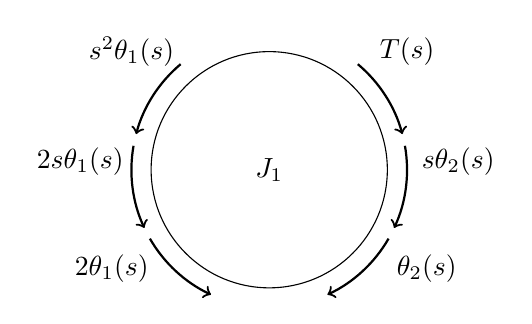
\begin{tikzpicture}
                    % Circle
                    \draw (0,0) circle (1.5);
                    \node at (0,0) {$J_1$};
                    % Left-hand Arrows
                    \draw[->, thick] (0,0) ++(130:1.75) arc[start angle=130, end angle=165, radius=1.75];
                    \node at (-1.75,1.5){$s^2\theta_1(s)$};
                    \draw[->, thick] (0,0) ++(170:1.75) arc[start angle=170, end angle=205, radius=1.75];
                    \node at (-2.4,0.1){$2s\theta_1(s)$};
                    \draw[->, thick] (0,0) ++(210:1.75) arc[start angle=210, end angle=245, radius=1.75];
                    \node at (-2,-1.25){$2\theta_1(s)$};
                    % Right-hand Arrows
                    \draw[->, thick] (0,0) ++(50:1.75) arc[start angle=50, end angle=15, radius=1.75];
                    \node at (1.75,1.5){$T(s)$};
                    \draw[->, thick] (0,0) ++(10:1.75) arc[start angle=10, end angle=-25, radius=1.75];
                    \node at (2.4,0.1){$s\theta_2(s)$};
                    \draw[->, thick] (0,0) ++(-30:1.75) arc[start angle=-30, end angle=-65, radius=1.75];
                    \node at (2,-1.25){$\theta_2(s)$};
                \end{tikzpicture}
        
                % Equations under J1
                \vspace{15pt}

                $\sum T_0 = 0 \quad\text{(clockwise, +)}$ \\ \vspace{10pt}
                $T(s) - (s^2+2s+2)\theta_1(s) + (s+1)\theta_2(s) = 0$ \\ \vspace{10pt}
                $T(s) = (s^2+2s+2)\theta_1(s) - (s+1)\theta_2(s)$

    \end{center}
\newpage
        \begin{center}
                \textbf{Free Body Diagram at $J_2$} \\[6pt]
				\vspace{15pt}
                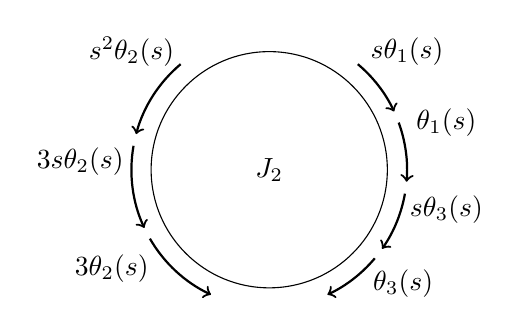
\begin{tikzpicture}
                    % Circle
                    \draw (0,0) circle (1.5);
                    \node at (0,0) {$J_2$};
                    % Left-hand Arrows
                    \draw[->, thick] (0,0) ++(130:1.75) arc[start angle=130, end angle=165, radius=1.75];
                    \node at (-1.75,1.5){$s^2\theta_2(s)$};
                    \draw[->, thick] (0,0) ++(170:1.75) arc[start angle=170, end angle=205, radius=1.75];
                    \node at (-2.4,0.1){$3s\theta_2(s)$};
                    \draw[->, thick] (0,0) ++(210:1.75) arc[start angle=210, end angle=245, radius=1.75];
                    \node at (-2,-1.25){$3\theta_2(s)$};
                    % Right-hand Arrows
                    \draw[->, thick] (0,0) ++(50:1.75) arc[start angle=50, end angle=25, radius=1.75];
                    \node at (1.75,1.5){$s\theta_1(s)$};
                    \draw[->, thick] (0,0) ++(20:1.75) arc[start angle=20, end angle=-5, radius=1.75];
                    \node at (2.25,0.6){$\theta_1(s)$};
                    \draw[->, thick] (0,0) ++(-10:1.75) arc[start angle=-10, end angle=-35, radius=1.75];
                    \node at (2.25,-0.5){$s\theta_3(s)$};
                    \draw[->, thick] (0,0) ++(-40:1.75) arc[start angle=-40, end angle=-65, radius=1.75];
                    \node at (1.7,-1.45){$\theta_3(s)$};
                \end{tikzpicture}
        
                % Equations under J2
        
        \vspace{15pt}
        

            $\sum T_0 = 0 \quad\text{(clockwise, +)}$ \\ \vspace{10pt}
            $0 = (s+1)\theta_1(s) - (s^2+3s+3)\theta_2(s) + (s+1)\theta_3(s)$ \\ \vspace{10pt}
            $0 = -(s+)\theta_1(s) + (s^2+3s+3)\theta_2(s) - (s+1)\theta_3(s)$

        
            \end{center}
    \vspace{15pt}
        \begin{center}
                \textbf{Free Body Diagram at $J_3$} \\[6pt]
				\vspace{15pt}
                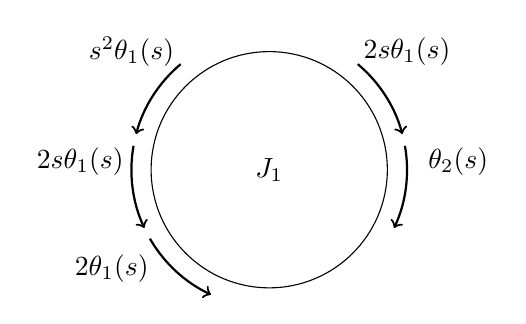
\begin{tikzpicture}
                    % Circle
                    \draw (0,0) circle (1.5);
                    \node at (0,0) {$J_1$};
                    % Left-hand Arrows
                    \draw[->, thick] (0,0) ++(130:1.75) arc[start angle=130, end angle=165, radius=1.75];
                    \node at (-1.75,1.5){$s^2\theta_1(s)$};
                    \draw[->, thick] (0,0) ++(170:1.75) arc[start angle=170, end angle=205, radius=1.75];
                    \node at (-2.4,0.1){$2s\theta_1(s)$};
                    \draw[->, thick] (0,0) ++(210:1.75) arc[start angle=210, end angle=245, radius=1.75];
                    \node at (-2,-1.25){$2\theta_1(s)$};
                    % Right-hand Arrows
                    \draw[->, thick] (0,0) ++(50:1.75) arc[start angle=50, end angle=15, radius=1.75];
                    \node at (1.75,1.5){$2s\theta_1(s)$};
                    \draw[->, thick] (0,0) ++(10:1.75) arc[start angle=10, end angle=-25, radius=1.75];
                    \node at (2.4,0.1){$\theta_2(s)$};
                  
                \end{tikzpicture}
        
                % Equations under J1
                \vspace{15pt}
        
                $\sum T_0 = 0 \quad\text{(clockwise, +)}$\\ \vspace{10pt}
                $0 = (s+1)\theta_2(s) - (s^2 + 2s + 2)\theta_3(s)$ \\ \vspace{10pt}
                $0 = -(s+1)\theta_2(s) + (s^2 + 2s + 2)\theta_3(s)$ 

    \end{center}

		\item Write the angular displacement equations and provide the matrix form
\begin{center}
	T(s) $= (s^2+2s+2)\theta_1(s) - (s+1)\theta_2(s)$\\
	0 $= -(s+1)\theta_1(s) + (s^2+3s+3)\theta_2(s) - (s+1)\theta_3(s)$\\
    0 $= -(s+1)\theta_2(s) + (s^2 + 2s + 2)\theta_3(s) $
	\[
		\begin{bmatrix}
		(s^2 + 2s + 2) & -(s+1) & 0\\
		-(s+1) & (s^2 + 3s + 3) & -(s+1)\\
        0 & -(s+1) & (s^2 + 2s + 2)
		\end{bmatrix}
		\begin{bmatrix}
		\theta_1(s) \\
		\theta_2(s) \\ 
        \theta_3(s)
		\end{bmatrix}
		=
		\begin{bmatrix}
		T(s)\\
		0 \\
        0
		\end{bmatrix}
	\]\\
\end{center}
		\item Apply Cramer's Rule to get the value of the Transfer Function
\begin{center}
	\[
		\theta_1(s) = 
			\frac{\begin{vmatrix}
				T(s) & -(s+1) & 0\\
		          0 & (s^2 + 3s + 3) & -(s+1)\\
                0 & -(s+1) & (s^2 + 2s + 2)
			\end{vmatrix}
		}{\begin{vmatrix}
				(s^2 + 2s + 2) & -(s+1) & 0\\
		          -(s+1) & (s^2 + 3s + 3) & -(s+1)\\
                0 & -(s+1) & (s^2 + 2s + 2)
			\end{vmatrix}
		}
	\]
	\[
	\theta_1(s) = \frac{(s^4 + 5s^3 + 10s^2 + 10s + 5)T(s)}{s^6 + 7s^5 + 21s^4 + 36s^3 + 38s^2 + 24s + 8}
	\] 

	\[
	\boxed{\frac{\theta_1(s)}{T(s)} = \frac{s^4 + 5s^3 + 10s^2 + 10s + 5}{s^6 + 7s^5 + 21s^4 + 36s^3 + 38s^2 + 24s + 8}}
	\]
\end{center}
	\end{enumerate}

% End of Problem 16

\end{fold}

% Problem 21
\begin{fold}
\newpage
% Problem 21

\newpage
\noindent\rule{\textwidth}{1pt}
\noindent\textbf{Problem 21} \hfill 
%palagay ulit dito 'yung problem statement
\\Solve for the Transfer Function, $\dfrac{\theta_1(s)}{T(s)}$, of the given Rotational Control System\\	
\begin{center}
\scalebox{0.95}{
	\begin{tikzpicture}[every node/.append style={font=\scriptsize}]
		% wall
		\def\brickw{0.24}   % brick width
		\def\brickh{0.18} % brick height
		\def\nrows{22}   % number of rows
		% draw bricks row by row
        \begin{scope}[shift={(-2,0)}]
		\foreach \r in {0,...,\nrows} {
			% shift every other row
			\pgfmathparse{mod(\r,2)==0 ? 0 : 0.5*\brickw}
			\let\shift\pgfmathresult
			\foreach \c in {0,1} {
			\draw[thick] (\shift+\c*\brickw, \r*\brickh) rectangle ++(\brickw,\brickh);
		}}
		\draw (0,0) rectangle (0.6,4.14);
        \end{scope}
        
        % spring
		\draw (-1.4,1.1) [cute inductor=] to (1.5,1.1);
		%Inertia
  		\draw (1.5,1.8) -- (4.1,1.8);
  		\draw (1.5,0.3) -- (4.1,0.3);
  		\draw (1.5,1.05) ellipse (0.15 and 0.75);
  		\draw (4.1,0.3) arc[start angle=-90, end angle=90, x radius=0.2, y radius=0.75];

        \begin{scope}[shift={(0,2.5)}]
            % spring
    		\draw (-1.4,1.1) [cute inductor=] to (1.5,1.1);
    		%Inertia
      		\draw (1.5,1.8) -- (4.1,1.8);
      		\draw (1.5,0.3) -- (4.1,0.3);
      		\draw (1.5,1.05) ellipse (0.15 and 0.75);
      		\draw (4.1,0.3) arc[start angle=-90, end angle=90, x radius=0.2, y radius=0.75];
        % spring
		\draw (4.3,0.65) [cute inductor=] to (6.2,0.65);
		% mass damper
		\draw (4.3,1.4) to (4.75,1.4);
            \begin{scope}[shift={(-0.25,0)}]
		\draw (5,1) to (5, 1.8);
		\draw (5,1) to (5.8, 1);
		\draw (5,1.8) to (5.8, 1.8);
		\draw (5.4, 1.2) to (5.4, 1.6);
            \end{scope}
		\draw (5.15,1.4) to (6.2, 1.4);
        \end{scope}
        
		% spring
		\draw (4.3,0.65) [cute inductor=] to (6.2,0.65);
		% mass damper
		\draw (4.3,1.4) to (4.75,1.4);
            \begin{scope}[shift={(-0.25,0)}]
		\draw (5,1) to (5, 1.8);
		\draw (5,1) to (5.8, 1);
		\draw (5,1.8) to (5.8, 1.8);
		\draw (5.4, 1.2) to (5.4, 1.6);
            \end{scope}
		\draw (5.15,1.4) to (6.2, 1.4);
		%Inertia
  		\draw (6.2,4.5) -- (8.8,4.5);
  		\draw (6.2,0) -- (8.8,0);
  		\draw (6.2,2.25) ellipse (0.2 and 2.25);
  		\draw (8.8,0) arc[start angle=-90, end angle=90, x radius=0.275, y radius=2.25];

		% spring
		\draw (9.05,1.65) [cute inductor=] to (12.4,1.65);
		% mass damper
		\draw (9.05,2.4) to (10.2,2.4);
            \begin{scope}[shift={(1,0)}]
		\draw (9.2,2) to (9.2, 2.8);
		\draw (9.2,2) to (10, 2);
		\draw (9.2,2.8) to (10, 2.8);
		\draw (9.6, 2.2) to (9.6, 2.6);
            \end{scope}
		\draw (10.6,2.4) to (12.4, 2.4);
		% wall
		\def\brickw{0.24}   % brick width
		\def\brickh{0.18} % brick height
		\def\nrows{22}   % number of rows
		% draw bricks row by row
		\begin{scope}[shift={(12.4,0)}]
			\foreach \r in {0,...,\nrows} {
				% shift every other row
				\pgfmathparse{mod(\r,2)==0 ? 0 : 0.5*\brickw}
				\let\shift\pgfmathresult
				\foreach \c in {0,1} {
				\draw[thick] (\shift+\c*\brickw, \r*\brickh) rectangle ++(\brickw,\brickh);
			}}
			\draw (0,0) rectangle (0.6,4.14);
		\end{scope}
		
	    % Label 1
		\node[scale=0.75] at (0.1, 0.7) {$2N-m/rad$};
		\node[scale=0.75] at (2.8, 1.05) {$1kg-m^2$};
        % Label 2
		\node[scale=0.75] at (4.65, 2) {$5N-m-s/rad$};
		\node[scale=0.75] at (4.75, 0) {$3N-m/rad$};
		\node[scale=0.75] at (7.65, 2.25) {$1kg-m^2$};
        % Label 3
        \begin{scope}[shift={(0,2.5)}]
    		\node[scale=0.75] at (0.1, 0.7) {$5N-m/rad$};
    		\node[scale=0.75] at (2.8, 1.05) {$kg-m^2$};
            \node[scale=0.75] at (4.65, 2) {$3N-m-s/rad$};
		    \node[scale=0.75] at (4.75, 0) {$2N-m/rad$};
        \end{scope}
		\node[scale=0.75] at (10.5, 3) {$5N-m-s/rad$};
		\node[scale=0.75] at (10.5, 1.25) {$3N-m/rad$};

		% Arrows 1
		\draw[<-,cyan] (3.75,1.8) arc[start angle=45,end angle=315,x radius=0.5,y radius=1.1];
		\node[cyan] at (3.5,-0.3) {$\theta_1(t)$};
		\draw[<-,cyan] (3,1.8) arc[start angle=45,end angle=315,x radius=0.5,y radius=1.1];
		\node[cyan] at (2.75,-0.3) {$T(t)$};
		% Arrows 2
		\draw[<-, cyan] (8.25,4.7) arc[start angle=60,end angle=300,x radius=0.5,y radius=2.8];
		\node[cyan] at (8.05,5.35) {$\theta_2(t)$};
        % Arrows 3
        \begin{scope}[shift={(0,2.5)}]
    		\draw[<-,cyan] (3.5,1.8) arc[start angle=45,end angle=315,x radius=0.5,y radius=1.1];
    		\node[cyan] at (3.25,2.45) {$\theta_3(t)$};
        \end{scope}
	\end{tikzpicture}
} % end scalebox
\end{center}


\noindent\rule{\textwidth}{1pt}

\noindent \textbf{\textit{Given:}}\\

\[
\begin{aligned}
J_1 &= 1\,\text{kg·m}^2 \qquad & f_{v1} &= 5\,\text{N·m·s/rad} \qquad & K_1 &= 2\,\text{N·m/rad} \\
J_2 &= 1\,\text{kg·m}^2 \qquad & f_{v2} &= 5\,\text{N·m·s/rad} \qquad & K_2 &= 3\,\text{N·m/rad} \\
J_3 &= 1\,\text{kg·m}^2 \qquad & f_{v3} &= 3\,\text{N·m·s/rad} \qquad & K_3 &= 3\,\text{N·m/rad} \\
&&& & K_4 &= 2\,\text{N·m/rad} \\
&&& & K_5 &= 5\,\text{N·m/rad}
\end{aligned}
\]


\noindent \textbf{\textit{Required:}}\\

\begin{center}
	$\dfrac{\theta_1(s)}{T(s)}$
\end{center}


\noindent \textbf{\textit{Solution:}}\\

	\begin{enumerate}[label=(\alph*),itemindent=*, itemindent=*, leftmargin=*, nolistsep]
		\item Draw the Free Body Diagram of the Inertias\\[6pt]

        \begin{center}
                \textbf{Free Body Diagram at $J_1$} \\[6pt]
				\vspace{15pt}
                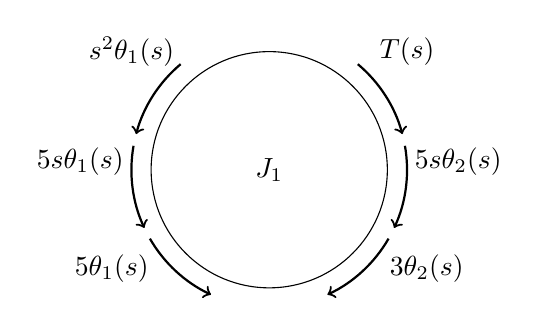
\begin{tikzpicture}
                    % Circle
                    \draw (0,0) circle (1.5);
                    \node at (0,0) {$J_1$};
                    % Left-hand Arrows
                    \draw[->, thick] (0,0) ++(130:1.75) arc[start angle=130, end angle=165, radius=1.75];
                    \node at (-1.75,1.5){$s^2\theta_1(s)$};
                    \draw[->, thick] (0,0) ++(170:1.75) arc[start angle=170, end angle=205, radius=1.75];
                    \node at (-2.4,0.1){$5s\theta_1(s)$};
                    \draw[->, thick] (0,0) ++(210:1.75) arc[start angle=210, end angle=245, radius=1.75];
                    \node at (-2,-1.25){$5\theta_1(s)$};
                    % Right-hand Arrows
                    \draw[->, thick] (0,0) ++(50:1.75) arc[start angle=50, end angle=15, radius=1.75];
                    \node at (1.75,1.5){$T(s)$};
                    \draw[->, thick] (0,0) ++(10:1.75) arc[start angle=10, end angle=-25, radius=1.75];
                    \node at (2.4,0.1){$5s\theta_2(s)$};
                    \draw[->, thick] (0,0) ++(-30:1.75) arc[start angle=-30, end angle=-65, radius=1.75];
                    \node at (2,-1.25){$3\theta_2(s)$};
                \end{tikzpicture}
        
                % Equations under J1
                \vspace{15pt}

            $\sum T_0 = 0 \quad\text{(clockwise, +)}$ \\ \vspace{10pt}
            $T(s) -(s^2+5s+5)\theta_1(s) + (5s+3)\theta_2(s) = 0$ \\ \vspace{10pt}
            $T(s) = (s^2+5s+5)\theta_1(s) - (5s+3)\theta_2(s)$

        \end{center}
        \vspace{15pt}
        \newpage
        \begin{center}
                \textbf{Free Body Diagram at $J_2$} \\[6pt]
				\vspace{15pt}
                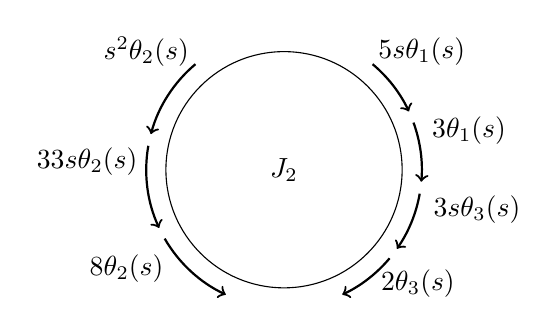
\begin{tikzpicture}
                    % Circle
                    \draw (0,0) circle (1.5);
                    \node at (0,0) {$J_2$};
                    % Left-hand Arrows
                    \draw[->, thick] (0,0) ++(130:1.75) arc[start angle=130, end angle=165, radius=1.75];
                    \node at (-1.75,1.5){$s^2\theta_2(s)$};
                    \draw[->, thick] (0,0) ++(170:1.75) arc[start angle=170, end angle=205, radius=1.75];
                    \node at (-2.5,0.1){$33s\theta_2(s)$};
                    \draw[->, thick] (0,0) ++(210:1.75) arc[start angle=210, end angle=245, radius=1.75];
                    \node at (-2,-1.25){$8\theta_2(s)$};
                    % Right-hand Arrows
                    \draw[->, thick] (0,0) ++(50:1.75) arc[start angle=50, end angle=25, radius=1.75];
                    \node at (1.75,1.5){$5s\theta_1(s)$};
                    \draw[->, thick] (0,0) ++(20:1.75) arc[start angle=20, end angle=-5, radius=1.75];
                    \node at (2.35,0.5){$3\theta_1(s)$};
                    \draw[->, thick] (0,0) ++(-10:1.75) arc[start angle=-10, end angle=-35, radius=1.75];
                    \node at (2.45,-0.5){$3s\theta_3(s)$};
                    \draw[->, thick] (0,0) ++(-40:1.75) arc[start angle=-40, end angle=-65, radius=1.75];
                    \node at (1.7,-1.45){$2\theta_3(s)$};
                \end{tikzpicture}
        
                % Equations under J2
        
        \vspace{15pt}
        
            $\sum T_0 = 0 \quad\text{(clockwise, +)}$ \\ \vspace{10pt}
            $0 = (5s+3)\theta_1(s) - (s^2+13s+8)\theta_2(s) + (3s+2)\theta_3(s)$ \\ \vspace{10pt}
            $0 = -(5s+3)\theta_1(s) + (s^2+13s+8)\theta_2(s) - (3s+2)\theta_3(s)$
        
		\end{center}
        \vspace{15pt}
        \begin{center}
                \textbf{Free Body Diagram at $J_3$} \\[6pt]
				\vspace{15pt}
                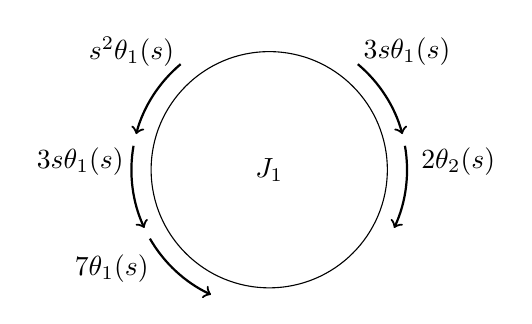
\begin{tikzpicture}
                    % Circle
                    \draw (0,0) circle (1.5);
                    \node at (0,0) {$J_1$};
                    % Left-hand Arrows
                    \draw[->, thick] (0,0) ++(130:1.75) arc[start angle=130, end angle=165, radius=1.75];
                    \node at (-1.75,1.5){$s^2\theta_1(s)$};
                    \draw[->, thick] (0,0) ++(170:1.75) arc[start angle=170, end angle=205, radius=1.75];
                    \node at (-2.4,0.1){$3s\theta_1(s)$};
                    \draw[->, thick] (0,0) ++(210:1.75) arc[start angle=210, end angle=245, radius=1.75];
                    \node at (-2,-1.25){$7\theta_1(s)$};
                    % Right-hand Arrows
                    \draw[->, thick] (0,0) ++(50:1.75) arc[start angle=50, end angle=15, radius=1.75];
                    \node at (1.75,1.5){$3s\theta_1(s)$};
                    \draw[->, thick] (0,0) ++(10:1.75) arc[start angle=10, end angle=-25, radius=1.75];
                    \node at (2.4,0.1){$2\theta_2(s)$};
                  
                \end{tikzpicture}
        
                % Equations under J1
                \vspace{15pt}
        

            $\sum T_0 = 0 \quad\text{(clockwise, +)}$ \\ \vspace{10pt}
            $0 = (3s+2)\theta_2(s) - (s^2 + 3s + 7)\theta_3(s)$ \\ \vspace{10pt}
            $0 = -(3s+2)\theta_2(s) + (s^2 + 3s + 7)\theta_3(s)$

            \end{center}

		\item Write the angular displacement equations and provide the matrix form
\begin{center}
	T(s) $= (s^2+5s+5)\theta_1(s) - (5s+3)\theta_2(s)$\\
	0 $= -(5s+3)\theta_1(s) + (s^2+13s+8)\theta_2(s) - (3s+2)\theta_3(s)$\\
    0 $= -(3s+2)\theta_2(s) + (s^2 + 3s + 7)\theta_3(s) $
	\[
		\begin{bmatrix}
		(s^2+5s+5) & -(5s+3) & 0\\
		-(5s+3) & (s^2 + 13s + 8) & -(3s+2)\\
        0 & -(3s+2) & (s^2 + 3s + 7)
		\end{bmatrix}
		\begin{bmatrix}
		\theta_1(s) \\
		\theta_2(s) \\ 
        \theta_3(s)
		\end{bmatrix}
		=
		\begin{bmatrix}
		T(s)\\
		0 \\
        0
		\end{bmatrix}
	\]\\
\end{center}
		\item Apply Cramer's Rule to get the value of the Transfer Function
\begin{center}
	\[
		\theta_1(s) = 
			\frac{\begin{vmatrix}
				T(s) & -(5s+3) & 0\\
		          0 & (s^2 + 13s + 8) & -(3s+2)\\
                0 & -(3s+2) & (s^2 + 3s + 7)
			\end{vmatrix}
		}{\begin{vmatrix}
				(s^2+5s+5) & -(5s+3) & 0\\
		          -(5s+3) & (s^2 + 13s + 8) & -(3s+2)\\
                0 & -(3s+2) & (s^2 + 3s + 7)
			\end{vmatrix}
		}
	\]
	\[
	\theta_1(s) = \frac{(s^4 + 16s^3 + 45s^2 + 103s + 52)T(s)}{s^6 + 21s^5 + 105s^4 + 303s^3 + 518s^2 + 538s + 197}
	\] 

	\[
	\boxed{\frac{\theta_1(s)}{T(s)} = \frac{s^4 + 16s^3 + 45s^2 + 103s + 52}{s^6 + 21s^5 + 105s^4 + 303s^3 + 518s^2 + 538s + 197}}
	\]
\end{center}
	\end{enumerate}

% End of Problem 21

\end{fold}

% Problem 22
\begin{fold}

\newpage
\noindent\rule{\textwidth}{1pt}
\noindent\textbf{Problem 22} \hfill 
\\Given the Rotational Mechanical System below, solve for the Transfer Function $\frac{\theta_1(s)}{F(s)}$\\

\begin{center}
	\begin{tikzpicture}[scale=0.7, every node/.style={font=\scriptsize}]
		% wall
            
		\def\brickw{0.24}   % brick width
		\def\brickh{0.18} % brick height
		\def\nrows{45}   % number of rows
		% draw bricks row by row
        \begin{scope}[shift={(-3,0)}]
		\foreach \r in {0,...,\nrows} {
			% shift every other row
			\pgfmathparse{mod(\r,2)==0 ? 0 : 0.5*\brickw}
			\let\shift\pgfmathresult
			\foreach \c in {0,1} {
			\draw[thick] (\shift+\c*\brickw, \r*\brickh) rectangle ++(\brickw,\brickh);
		}}
		\draw (0,0) rectangle (0.6,8.28);
        
            \end{scope}
		% spring
		\draw (-2.4,0.5) [cute inductor=] to (0.75,0.5);
		% mass damper
		\draw (-2.4,1.4) to (-1.2,1.4);
            \begin{scope}[shift={(-2,0)}]
		\draw (0.8,1) to (0.8, 1.8);
		\draw (0.8,1) to (1.6, 1);
		\draw (0.8,1.8) to (1.6, 1.8);
		\draw (1.2, 1.2) to (1.2, 1.6);
            \end{scope}
		\draw (-0.8,1.4) to (0.75, 1.4);
        \begin{scope}[shift={(-0.75,0)}]
		    %Inertia
            \draw (1.5,1.8) -- (4.1,1.8);
            \draw (1.5,0.3) -- (4.1,0.3);
            \draw (1.5,1.05) ellipse (0.15 and 0.75);
            \draw (4.1,0.3) arc[start angle=-90, end angle=90, x                radius=0.2, y radius=0.75];
        \end{scope}
        \begin{scope}[shift={(-0.5,0)}]
            % spring
            \draw (4,0.5) [cute inductor=] to (6.55,0.5);
            % mass damper
            \draw (4,1.4) to (4.75,1.4);
                \begin{scope}[shift={(-0.25,0)}]
            \draw (5,1) to (5, 1.8);
            \draw (5,1) to (5.8, 1);
            \draw (5,1.8) to (5.8, 1.8);
            \draw (5.4, 1.2) to (5.4, 1.6);
                \end{scope}
            \draw (5.15,1.4) to (6.55, 1.4);
            \end{scope}
		%Inertia
  		\draw (6.2,5) -- (8.8,5);
  		\draw (6.2,0) -- (8.8,0);
  		\draw (6.2,2.5) ellipse (0.2 and 2.5);
  		\draw (8.8,0) arc[start angle=-90, end angle=90, x radius=0.275, y radius=2.5];
        % long damper and spring
        \draw (-2.4,3.75) [cute inductor=] to (6.2,3.75);
		% mass damper
        \begin{scope}[shift={(-1,0.9)}]
            \draw (-1.4,3.75) to (2.5,3.75);
                \begin{scope}[shift={(-0.5,0)}]
            \draw (3.05,3.35) to (3.05, 4.15);
            \draw (3.05,3.35) to (3.85, 3.35);
            \draw (3.05,4.15) to (3.85, 4.15);
            \draw (3.45, 3.55) to (3.45, 3.95);
                \end{scope}
            \draw (2.95,3.75) to (7.2, 3.75);
        \end{scope}

		% spring
        \draw (9.05,1.25) [cute inductor=] to (12.4,1.25);
    	% mass damper
    	\draw (9.05,4) to (10.2,4);
            \begin{scope}[shift={(1,1.6)}]
    	\draw (9.2,2) to (9.2, 2.8);
    	\draw (9.2,2) to (10, 2);
    	\draw (9.2,2.8) to (10, 2.8);
    	\draw (9.6, 2.2) to (9.6, 2.6);
            \end{scope}
    	\draw (10.6,4) to (12.4, 4);
        %Inertia
  		\draw (12.4,9) -- (15,9);
  		\draw (12.4,0) -- (15,0);
  		\draw (12.4,4.5) ellipse (0.2 and 4.5);
  		\draw (15,0) arc[start angle=-90, end angle=90, x                radius=0.275, y radius=4.5];
       	\begin{scope}[shift={(6.2,2.25)}]
            % spring
            \draw (9.05,1) [cute inductor=] to (12.4,1);
        	% mass damper
        	\draw (9.05,3) to (10.2,3);
                \begin{scope}[shift={(1,0.6)}]
        	\draw (9.2,2) to (9.2, 2.8);
        	\draw (9.2,2) to (10, 2);
        	\draw (9.2,2.8) to (10, 2.8);
        	\draw (9.6, 2.2) to (9.6, 2.6);
                \end{scope}
        	\draw (10.6,3) to (12.4, 3);
        \end{scope}
        \begin{scope}[shift={(-1,3.5)}]
            % long damper and spring
            \draw (-1.4,3.2) [cute inductor=] to (13.2,3.2);
    		% mass damper
    		\draw (-1.4,4.25) to (5.3,4.25);
                \begin{scope}[shift={(2.25,0.5)}]
    		\draw (3.05,3.35) to (3.05, 4.15);
    		\draw (3.05,3.35) to (3.85, 3.35);
    		\draw (3.05,4.15) to (3.85, 4.15);
    		\draw (3.45, 3.55) to (3.45, 3.95);
                \end{scope}
    		\draw (5.7,4.25) to (13.5, 4.25);
        \end{scope}
		% wall
		\def\brickw{0.24}   % brick width
		\def\brickh{0.18} % brick height
		\def\nrows{45}   % number of rows
		% draw bricks row by row
		\begin{scope}[shift={(18.62,0)}]
			\foreach \r in {0,...,\nrows} {
				% shift every other row
				\pgfmathparse{mod(\r,2)==0 ? 0 : 0.5*\brickw}
				\let\shift\pgfmathresult
				\foreach \c in {0,1} {
				\draw[thick] (\shift+\c*\brickw, \r*\brickh) rectangle ++(\brickw,\brickh);
			}}
			\draw (0,0) rectangle (0.61,8.28);
		\end{scope}
		
	    % Label 1
		\node at (-0.75, 2.2) {$1N-m-s/rad$};
		\node at (-0.75, 0) {$1N-m/rad$};
		\node at (2.1, 1.05) {$1kg-m^2$};
        % Label 2
		\node at (4.5, 2.2) {$1N\cdot m\cdot s/rad$};
		\node at (4.75, 0) {$1N-m/rad$};
		\node at (7.65, 2.5) {$1kg-m^2$};
        \node at (2, 5.4) {$1N-m-s/rad$};
        \node at (2, 3.25) {$1N-m/rad$};
        % Label 3
		\node at (10.5, 3.25) {$1 N\cdot m\cdot s/rad$};
		\node at (10.5, 0.75) {$1 N-m/rad$};
        \begin{scope}[shift={(6.2,2.25)}]
            \node at (10.6, 3.8) {$1 N\cdot m\cdot s/rad$};
    		\node at (10.5, 0.4) {$1 N-m/rad$};
        \end{scope}
        \node at (14,4.5) {$1kg-m^2$};
        \node at (4.6,8.6) {$1N-m-s/rad$};
        \node at (4.75,6.15) {$1N-m/rad$};

        \begin{scope}[shift={(-0.75,0)}]
            % Arrows 1
            \draw[<-,cyan] (3.75,1.8) arc[start angle=45,end angle=315,x radius=0.5,y radius=1.1];
            \node[cyan] at (3.5,-0.35) {$\theta_1(t)$};
            \draw[<-,cyan] (3,1.8) arc[start angle=45,end angle=315,x radius=0.5,y radius=1.1];
            \node[cyan] at (2.55,-0.35) {$T(t)$};
        \end{scope}
		% Arrows 2
		\draw[<-, cyan] (8,5.25) arc[start angle=60,end angle=300,x radius=0.5,y radius=3.3];
		\node[cyan] at (7.8,6) {$\theta_2(t)$};
        % Arrows 3
        \draw[<-, cyan] (14.25,9.1) arc[start angle=60,end angle=300,x radius=0.5,y radius=5.3];
		\node[cyan] at (14,10.1) {$\theta_3(t)$};
	\end{tikzpicture}
\end{center}
\noindent\rule{\textwidth}{1pt}\\

\noindent \textbf{\textit{Given:}}\\

\[
\begin{aligned}
J_1 &= 1\,\text{kg·m}^2 \qquad & f_{v1} &= 1\,\text{N·m·s/rad} \qquad & K_1 &= 1\,\text{N·m/rad} \\
J_2 &= 1\,\text{kg·m}^2 \qquad & f_{v2} &= 1\,\text{N·m·s/rad} \qquad & K_2 &= 1\,\text{N·m/rad} \\
J_3 &= 1\,\text{kg·m}^2 \qquad & f_{v3} &= 1\,\text{N·m·s/rad} \qquad & K_3 &= 1\,\text{N·m/rad} \\
&& f_{v4} &= 1\,\text{N·m·s/rad} \qquad & K_4 &= 1\,\text{N·m/rad} \\
&& f_{v5} &= 1\,\text{N·m·s/rad} \qquad & K_5 &= 1\,\text{N·m/rad} \\
&& f_{v6} &= 1\,\text{N·m·s/rad} \qquad & K_6 &= 1\,\text{N·m/rad}
\end{aligned}
\]


\noindent \textbf{\textit{Required:}}\\

\begin{center}
	$\dfrac{\theta_1(s)}{T(s)}$
\end{center}

	\noindent \textbf{\textit{Solution:}}\\

	% Start of Solution
	\begin{enumerate}[label=(\alph*),itemindent=*, itemindent=*, leftmargin=*, nolistsep]
		
		\item Draw the Free Body Diagrams of the provided masses
	\vspace{10pt}
		\begin{center}
                \textbf{Free Body Diagram at $J_1$} \\[6pt]
				\vspace{15pt}
                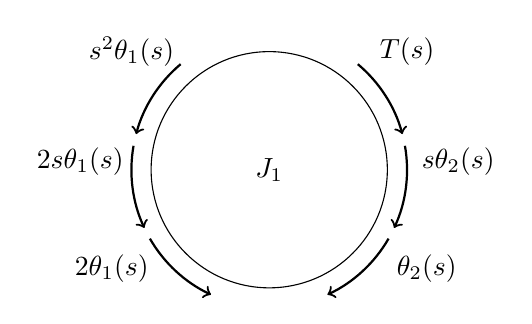
\begin{tikzpicture}
                    % Circle
                    \draw (0,0) circle (1.5);
                    \node at (0,0) {$J_1$};
                    % Left-hand Arrows
                    \draw[->, thick] (0,0) ++(130:1.75) arc[start angle=130, end angle=165, radius=1.75];
                    \node at (-1.75,1.5){$s^2\theta_1(s)$};
                    \draw[->, thick] (0,0) ++(170:1.75) arc[start angle=170, end angle=205, radius=1.75];
                    \node at (-2.4,0.1){$2s\theta_1(s)$};
                    \draw[->, thick] (0,0) ++(210:1.75) arc[start angle=210, end angle=245, radius=1.75];
                    \node at (-2,-1.25){$2\theta_1(s)$};
                    % Right-hand Arrows
                    \draw[->, thick] (0,0) ++(50:1.75) arc[start angle=50, end angle=15, radius=1.75];
                    \node at (1.75,1.5){$T(s)$};
                    \draw[->, thick] (0,0) ++(10:1.75) arc[start angle=10, end angle=-25, radius=1.75];
                    \node at (2.4,0.1){$s\theta_2(s)$};
                    \draw[->, thick] (0,0) ++(-30:1.75) arc[start angle=-30, end angle=-65, radius=1.75];
                    \node at (2,-1.25){$\theta_2(s)$};
                \end{tikzpicture}
        
                % Equations under J1
                \vspace{15pt}
        
                $\sum T_0 = 0 \quad\text{(clockwise, +)}$ \\ \vspace{10pt}
                $T(s) -(s^2+2s+2)\theta_1(s) + (s+1)\theta_2(s) = 0$ \\ \vspace{10pt}
                $T(s) = (s^2+2s+2)\theta_1(s) - (s+1)\theta_2(s)$

        \end{center}

    \vspace{15pt}
        \begin{center}
            %---------------- RIGHT SIDE: J2 ----------------%
                \textbf{Free Body Diagram at $J_2$} \\[6pt]
				\vspace{15pt}
                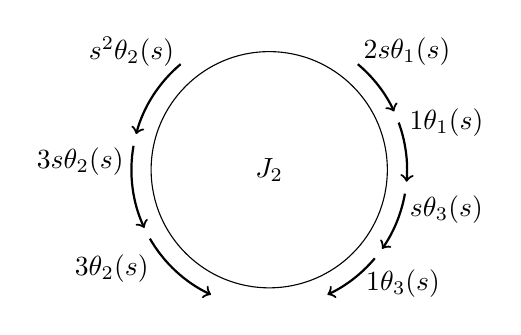
\begin{tikzpicture}
                    % Circle
                    \draw (0,0) circle (1.5);
                    \node at (0,0) {$J_2$};
                    % Left-hand Arrows
                    \draw[->, thick] (0,0) ++(130:1.75) arc[start angle=130, end angle=165, radius=1.75];
                    \node at (-1.75,1.5){$s^2\theta_2(s)$};
                    \draw[->, thick] (0,0) ++(170:1.75) arc[start angle=170, end angle=205, radius=1.75];
                    \node at (-2.4,0.1){$3s\theta_2(s)$};
                    \draw[->, thick] (0,0) ++(210:1.75) arc[start angle=210, end angle=245, radius=1.75];
                    \node at (-2,-1.25){$3\theta_2(s)$};
                    % Right-hand Arrows
                    \draw[->, thick] (0,0) ++(50:1.75) arc[start angle=50, end angle=25, radius=1.75];
                    \node at (1.75,1.5){$2s\theta_1(s)$};
                    \draw[->, thick] (0,0) ++(20:1.75) arc[start angle=20, end angle=-5, radius=1.75];
                    \node at (2.25,0.6){$1\theta_1(s)$};
                    \draw[->, thick] (0,0) ++(-10:1.75) arc[start angle=-10, end angle=-35, radius=1.75];
                    \node at (2.25,-0.5){$s\theta_3(s)$};
                    \draw[->, thick] (0,0) ++(-40:1.75) arc[start angle=-40, end angle=-65, radius=1.75];
                    \node at (1.7,-1.45){$1\theta_3(s)$};
                \end{tikzpicture}
        
                % Equations under J2
        
        \vspace{15pt}
        

            $\sum T_0 = 0 \quad\text{(clockwise, +)}$ \\ \vspace{10pt}
            $0 = (s+1)\theta_1(s) - (s^2+3s+3)\theta_2(s) + (s+1)\theta_3(s)$\\ \vspace{10pt}
            $0 = -(s+1)\theta_1(s) + (s^2+3s+3)\theta_2(s) - (s+1)\theta_3(s)$

        \end{center}

        \vspace{15pt}
        \begin{center}
                \textbf{Free Body Diagram at $J_3$} \\[6pt]
				\vspace{15pt}
                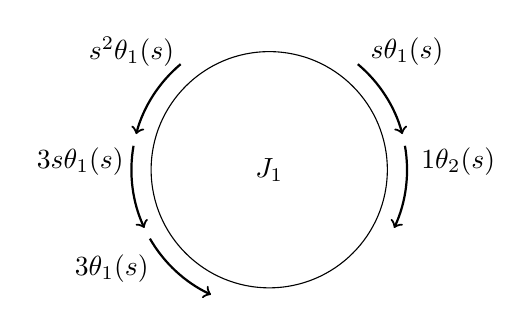
\begin{tikzpicture}
                    % Circle
                    \draw (0,0) circle (1.5);
                    \node at (0,0) {$J_1$};
                    % Left-hand Arrows
                    \draw[->, thick] (0,0) ++(130:1.75) arc[start angle=130, end angle=165, radius=1.75];
                    \node at (-1.75,1.5){$s^2\theta_1(s)$};
                    \draw[->, thick] (0,0) ++(170:1.75) arc[start angle=170, end angle=205, radius=1.75];
                    \node at (-2.4,0.1){$3s\theta_1(s)$};
                    \draw[->, thick] (0,0) ++(210:1.75) arc[start angle=210, end angle=245, radius=1.75];
                    \node at (-2,-1.25){$3\theta_1(s)$};
                    % Right-hand Arrows
                    \draw[->, thick] (0,0) ++(50:1.75) arc[start angle=50, end angle=15, radius=1.75];
                    \node at (1.75,1.5){$s\theta_1(s)$};
                    \draw[->, thick] (0,0) ++(10:1.75) arc[start angle=10, end angle=-25, radius=1.75];
                    \node at (2.4,0.1){$1\theta_2(s)$};
                  
                \end{tikzpicture}
        
                % Equations under J1
                \vspace{15pt}
        
                $\sum T_0 = 0 \quad\text{(clockwise, +)}$ \\ \vspace{10pt}
                $0 = (s+1)\theta_2(s) - (s^2 + 3s + 3)\theta_3(s)$ \\ \vspace{10pt}
                $0 = -(s+1)\theta_2(s) + (s^2 + 3s + 3)\theta_3(s)$ 

        \end{center}
\vspace{15pt}
		\item Write the displacement equations and provide the matrix form
\begin{center}
	T(s) $= (s^2 + 2s + 2)\theta_1(s) - (s + 1)\theta_2(s)$\\
	0 $= -(s + 1)\theta_1(s) + (s^2 + 3s + 3)\theta_2(s) -(s+1)\theta_3(s)$\\
	0 $= -(s + 1)\theta_2(s) + (s^2 + 3s + 3)\theta_3(s)$\\
	\[
		\begin{bmatrix}
		(s^2 + 2s + 2) & -(s + 1) & 0\\
		-(s + 1) & (s^2 + 3s + 3) & -(s+1)\\
		0 & -(s-1) & (s^2 + 3s +3)\\
		\end{bmatrix}
		\begin{bmatrix}
		\theta_1(s) \\
		\theta_2(s) \\
		\theta_3(s)
		\end{bmatrix}
		=
		\begin{bmatrix}
		T(s)\\
		0\\
		0
		\end{bmatrix}
	\]\\
\end{center}
\vspace{15pt}
		\item Apply Cramer's Rule to get the value of the Transfer Function
\begin{center}
	\[
		\theta_1(s) = 
			\frac{\begin{vmatrix}
				T(s) & -(s + 1) & 0\\
				0 & (s^2 + 3s + 3) & -(s+1)\\
				0 & -(s-1) & (s^2 + 3s + 3)\\
			\end{vmatrix}
		}{\begin{vmatrix}
				(s^2 + 2s + 2) & -(s + 1) & 0\\
				-(s + 1) & (s^2 + 3s + 3) & -(s+1)\\
				0 & -(s-1) & (s^2 + 3s + 3)\\
			\end{vmatrix}
		}
	\]
	\[
	\theta_1(s) = \frac{(s^4 + 6s^3 + 14s^2 + 18s + 10)T(s)}{s^6 + 8s^5 + 27s^4 + 53s^3 + 64s^2 + 47s + 17}
	\] 

	\[
	\boxed{\frac{X_1(s)}{F(s)} = \frac{s^4 + 6^3 + 14s^2 + 18s + 10}{s^6 + 8s^5 + 27s^4 + 53s^3 + 64s^2 + 47s + 17}}
	\] 

\end{center}
	\end{enumerate}


\end{fold}

% Problem 23
\begin{fold}

\newpage
\noindent\rule{\textwidth}{1pt}
\noindent\textbf{Problem 23} \hfill 
\\Given the Rotational Mechanical System below, solve for the Transfer Function $\frac{\theta_1(s)}{F(s)}$\\

\begin{center}
	\begin{tikzpicture}[scale=0.7, every node/.style={font=\scriptsize}]
		% wall
            
		\def\brickw{0.24}   % brick width
		\def\brickh{0.18} % brick height
		\def\nrows{45}   % number of rows
		% draw bricks row by row
        \begin{scope}[shift={(-3,0)}]
		\foreach \r in {0,...,\nrows} {
			% shift every other row
			\pgfmathparse{mod(\r,2)==0 ? 0 : 0.5*\brickw}
			\let\shift\pgfmathresult
			\foreach \c in {0,1} {
			\draw[thick] (\shift+\c*\brickw, \r*\brickh) rectangle ++(\brickw,\brickh);
		}}
		\draw (0,0) rectangle (0.6,8.28);
        
            \end{scope}
		% spring
		\draw (-2.4,1) [cute inductor=] to (0.75,1);
        \begin{scope}[shift={(-0.75,0)}]
		    %Inertia
            \draw (1.5,1.8) -- (4.1,1.8);
            \draw (1.5,0.3) -- (4.1,0.3);
            \draw (1.5,1.05) ellipse (0.15 and 0.75);
            \draw (4.1,0.3) arc[start angle=-90, end angle=90, x                radius=0.2, y radius=0.75];
        \end{scope}
        \begin{scope}[shift={(-0.5,0)}]
            % spring
            \draw (4,0.5) [cute inductor=] to (6.55,0.5);
            % mass damper
            \draw (4,1.4) to (4.75,1.4);
                \begin{scope}[shift={(-0.25,0)}]
            \draw (5,1) to (5, 1.8);
            \draw (5,1) to (5.8, 1);
            \draw (5,1.8) to (5.8, 1.8);
            \draw (5.4, 1.2) to (5.4, 1.6);
                \end{scope}
            \draw (5.15,1.4) to (6.55, 1.4);
            \end{scope}
		%Inertia
  		\draw (6.2,5) -- (8.8,5);
  		\draw (6.2,0) -- (8.8,0);
  		\draw (6.2,2.5) ellipse (0.2 and 2.5);
  		\draw (8.8,0) arc[start angle=-90, end angle=90, x radius=0.275, y radius=2.5];
        % long damper and spring
        \draw (-2.4,3.75) [cute inductor=] to (6.2,3.75);
		% mass damper
        \begin{scope}[shift={(-1,0.9)}]
            \draw (-1.4,3.75) to (2.5,3.75);
                \begin{scope}[shift={(-0.5,0)}]
            \draw (3.05,3.35) to (3.05, 4.15);
            \draw (3.05,3.35) to (3.85, 3.35);
            \draw (3.05,4.15) to (3.85, 4.15);
            \draw (3.45, 3.55) to (3.45, 3.95);
                \end{scope}
            \draw (2.95,3.75) to (7.2, 3.75);
        \end{scope}

		% spring
        \draw (9.05,1.25) [cute inductor=] to (12.4,1.25);
    	% mass damper
    	\draw (9.05,4) to (10.2,4);
            \begin{scope}[shift={(1,1.6)}]
    	\draw (9.2,2) to (9.2, 2.8);
    	\draw (9.2,2) to (10, 2);
    	\draw (9.2,2.8) to (10, 2.8);
    	\draw (9.6, 2.2) to (9.6, 2.6);
            \end{scope}
    	\draw (10.6,4) to (12.4, 4);
        %Inertia
  		\draw (12.4,9) -- (15,9);
  		\draw (12.4,0) -- (15,0);
  		\draw (12.4,4.5) ellipse (0.2 and 4.5);
  		\draw (15,0) arc[start angle=-90, end angle=90, x                radius=0.275, y radius=4.5];
       	\begin{scope}[shift={(6.2,2.25)}]
            % spring
            \draw (9.05,1) [cute inductor=] to (12.4,1);
        	% mass damper
        	\draw (9.05,3) to (10.2,3);
                \begin{scope}[shift={(1,0.6)}]
        	\draw (9.2,2) to (9.2, 2.8);
        	\draw (9.2,2) to (10, 2);
        	\draw (9.2,2.8) to (10, 2.8);
        	\draw (9.6, 2.2) to (9.6, 2.6);
                \end{scope}
        	\draw (10.6,3) to (12.4, 3);
        \end{scope}
        \begin{scope}[shift={(-1,4.5)}]
            % long damper and spring
            \draw (-1.4,3.2) [cute inductor=] to (13.4,3.2);
        \end{scope}
		% wall
		\def\brickw{0.24}   % brick width
		\def\brickh{0.18} % brick height
		\def\nrows{45}   % number of rows
		% draw bricks row by row
		\begin{scope}[shift={(18.62,0)}]
			\foreach \r in {0,...,\nrows} {
				% shift every other row
				\pgfmathparse{mod(\r,2)==0 ? 0 : 0.5*\brickw}
				\let\shift\pgfmathresult
				\foreach \c in {0,1} {
				\draw[thick] (\shift+\c*\brickw, \r*\brickh) rectangle ++(\brickw,\brickh);
			}}
			\draw (0,0) rectangle (0.61,8.28);
		\end{scope}
		
		% Label 1
		\node at (-0.9, 1.6) {$7N-m/rad$};
		\node at (2.25, 1.05) {$5kg\cdot m^2$};
        % Label 2
		\node at (4.5, 2.2) {$9N\cdot m \cdot s/rad$};
		\node at (4.65, 0) {$6N-m/rad$};
		\node at (7.65, 2.5) {$8kg\cdot m^2$};
        \node at (2, 5.4) {$7N-m-s/rad$};
        \node at (1.9, 3.1) {$9N-m/rad$};
        % Label 3
		\node at (10.65, 3.1) {$5N\cdot m \cdot s/rad$};
		\node at (10.65, 0.65) {$8N-m/rad$};
        \begin{scope}[shift={(6.2,2.25)}]
            \node at (10.65, 3.75) {$6N\cdot m \cdot s/rad$};
    		\node at (10.5, 0.5) {$9N-m/rad$};
        \end{scope}
        \node at (14,4.5) {$5kg\cdot m^2$};
        \node at (4.9,8.45) {$8N-m/rad$};

        \begin{scope}[shift={(-0.75,0)}]
            % Arrows 1
            \draw[<-,cyan] (3.75,1.8) arc[start angle=45,end angle=315,x radius=0.5,y radius=1.1];
            \node[cyan] at (3.5,-0.35) {$\theta_1(t)$};
            \draw[<-,cyan] (3,1.8) arc[start angle=45,end angle=315,x radius=0.5,y radius=1.1];
            \node[cyan] at (2.55,-0.35) {$T(t)$};
        \end{scope}
		% Arrows 2
		\draw[<-, cyan] (8,5.25) arc[start angle=60,end angle=300,x radius=0.5,y radius=3.3];
		\node[cyan] at (7.8,6) {$\theta_2(t)$};
        % Arrows 3
        \draw[<-, cyan] (14.25,9.1) arc[start angle=60,end angle=300,x radius=0.5,y radius=5.3];
		\node[cyan] at (14,10.1) {$\theta_3(t)$};
	\end{tikzpicture}
\end{center}
\noindent\rule{\textwidth}{1pt}\\

\noindent \textbf{\textit{Given:}}\\

\[
\begin{aligned}
J_1 &= 1\,\text{kg·m}^2 \qquad & f_{v1} &= 9\,\text{N·m·s/rad} \qquad & K_1 &= 7\,\text{N·m/rad} \\
J_2 &= 1\,\text{kg·m}^2 \qquad & f_{v2} &= 5\,\text{N·m·s/rad} \qquad & K_2 &= 6\,\text{N·m/rad} \\
J_3 &= 1\,\text{kg·m}^2 \qquad & f_{v3} &= 7\,\text{N·m·s/rad} \qquad & K_3 &= 8\,\text{N·m/rad} \\
&& f_{v4} &= 6\,\text{N·m·s/rad} \qquad & K_4 &= 9\,\text{N·m/rad} \\
&&& & K_5 &= 9\,\text{N·m/rad} \\
&&& & K_6 &= 81\,\text{N·m/rad}
\end{aligned}
\]


\noindent \textbf{\textit{Required:}}\\

\begin{center}
	$\dfrac{\theta_1(s)}{T(s)}$
\end{center}

	\noindent \textbf{\textit{Solution:}}\\

	% Start of Solution
	\begin{enumerate}[label=(\alph*),itemindent=*, itemindent=*, leftmargin=*, nolistsep]
		\item Draw the Free Body Diagrams of the provided masses
	\vspace{15pt}
		\begin{center}
                \textbf{Free Body Diagram at $J_1$} \\[6pt]
                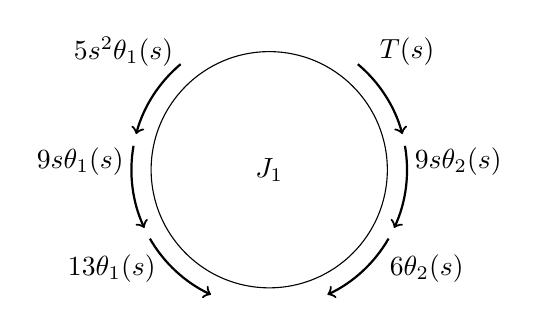
\begin{tikzpicture}
                    % Circle
                    \draw (0,0) circle (1.5);
                    \node at (0,0) {$J_1$};
                    % Left-hand Arrows
                    \draw[->, thick] (0,0) ++(130:1.75) arc[start angle=130, end angle=165, radius=1.75];
                    \node at (-1.85,1.5){$5s^2\theta_1(s)$};
                    \draw[->, thick] (0,0) ++(170:1.75) arc[start angle=170, end angle=205, radius=1.75];
                    \node at (-2.4,0.1){$9s\theta_1(s)$};
                    \draw[->, thick] (0,0) ++(210:1.75) arc[start angle=210, end angle=245, radius=1.75];
                    \node at (-2,-1.25){$13\theta_1(s)$};
                    % Right-hand Arrows
                    \draw[->, thick] (0,0) ++(50:1.75) arc[start angle=50, end angle=15, radius=1.75];
                    \node at (1.75,1.5){$T(s)$};
                    \draw[->, thick] (0,0) ++(10:1.75) arc[start angle=10, end angle=-25, radius=1.75];
                    \node at (2.4,0.1){$9s\theta_2(s)$};
                    \draw[->, thick] (0,0) ++(-30:1.75) arc[start angle=-30, end angle=-65, radius=1.75];
                    \node at (2,-1.25){$6\theta_2(s)$};
                \end{tikzpicture}
        
                % Equations under J1
                \vspace{15pt}

                $\sum T_0 = 0 \quad\text{(clockwise, +)}$ \\ \vspace{10pt}
                $T(s) -(8s^2+9s+13)\theta_1(s) + (9s+6)\theta_2(s) = 0$ \\ \vspace{10pt}
                $T(s) = (8s^2+9s+13)\theta_1(s) - (9s+6)\theta_2(s)$

            \end{center}

		\vspace{15pt}
        \begin{center}
                \textbf{Free Body Diagram at $J_2$} \\[6pt]
				\vspace{15pt}
                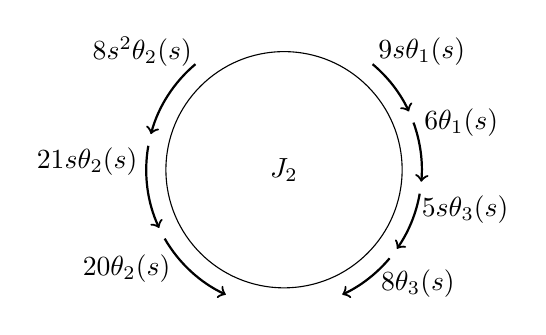
\begin{tikzpicture}
                    % Circle
                    \draw (0,0) circle (1.5);
                    \node at (0,0) {$J_2$};
                    % Left-hand Arrows
                    \draw[->, thick] (0,0) ++(130:1.75) arc[start angle=130, end angle=165, radius=1.75];
                    \node at (-1.80,1.5){$8s^2\theta_2(s)$};
                    \draw[->, thick] (0,0) ++(170:1.75) arc[start angle=170, end angle=205, radius=1.75];
                    \node at (-2.5,0.1){$21s\theta_2(s)$};
                    \draw[->, thick] (0,0) ++(210:1.75) arc[start angle=210, end angle=245, radius=1.75];
                    \node at (-2,-1.25){$20\theta_2(s)$};
                    % Right-hand Arrows
                    \draw[->, thick] (0,0) ++(50:1.75) arc[start angle=50, end angle=25, radius=1.75];
                    \node at (1.75,1.5){$9s\theta_1(s)$};
                    \draw[->, thick] (0,0) ++(20:1.75) arc[start angle=20, end angle=-5, radius=1.75];
                    \node at (2.25,0.6){$6\theta_1(s)$};
                    \draw[->, thick] (0,0) ++(-10:1.75) arc[start angle=-10, end angle=-35, radius=1.75];
                    \node at (2.30,-0.5){$5s\theta_3(s)$};
                    \draw[->, thick] (0,0) ++(-40:1.75) arc[start angle=-40, end angle=-65, radius=1.75];
                    \node at (1.7,-1.45){$8\theta_3(s)$};
                \end{tikzpicture}
        
                % Equations under J2
        
        \vspace{15pt}
        
                $\sum T_0 = 0 \quad\text{(clockwise, +)}$ \\ \vspace{10pt}
                $0 = (9s+6)\theta_1(s) - (8s^2+21s+20)\theta_2(s) + (5s+8)\theta_3(s)$ \\ \vspace{10pt}
                $0 = -(9s+6)\theta_1(s) + (8s^2+21s+20)\theta_2(s) - (5s+8)\theta_3(s)$
        
        \end{center}

		\vspace{15pt}
        
        \begin{center}
                \textbf{Free Body Diagram at $J_3$} \\[6pt]
				\vspace{15pt}
                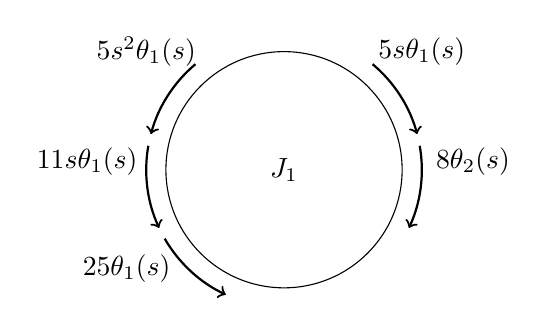
\begin{tikzpicture}
                    % Circle
                    \draw (0,0) circle (1.5);
                    \node at (0,0) {$J_1$};
                    % Left-hand Arrows
                    \draw[->, thick] (0,0) ++(130:1.75) arc[start angle=130, end angle=165, radius=1.75];
                    \node at (-1.75,1.5){$5s^2\theta_1(s)$};
                    \draw[->, thick] (0,0) ++(170:1.75) arc[start angle=170, end angle=205, radius=1.75];
                    \node at (-2.5,0.1){$11s\theta_1(s)$};
                    \draw[->, thick] (0,0) ++(210:1.75) arc[start angle=210, end angle=245, radius=1.75];
                    \node at (-2,-1.25){$25\theta_1(s)$};
                    % Right-hand Arrows
                    \draw[->, thick] (0,0) ++(50:1.75) arc[start angle=50, end angle=15, radius=1.75];
                    \node at (1.75,1.5){$5s\theta_1(s)$};
                    \draw[->, thick] (0,0) ++(10:1.75) arc[start angle=10, end angle=-25, radius=1.75];
                    \node at (2.4,0.1){$8\theta_2(s)$};
                  
                \end{tikzpicture}
        
                % Equations under J1
                \vspace{15pt}

                $\sum T_0 = 0 \quad\text{(clockwise, +)}$ \\ \vspace{10pt}
                $0 = (5s+8)\theta_2(s) - (5s^2 + 11s + 25)\theta_3(s)$ \\ \vspace{10pt}
                $0 = -(5s+8)\theta_2(s) + (5s^2 + 11s + 25)\theta_3(s) $

            \end{center}
	
		\item Write the displacement equations and provide the matrix form
\begin{center}
	T(s) $= (8s^2 + 9s + 13)\theta_1(s) - (9s + 6)\theta_2(s)$\\
	0 $= -(9s + 6)\theta_1(s) + (8s^2 + 21s + 20)\theta_2(s) -(5s+8)\theta_3(s)$\\
	0 $= -(5s + 8)\theta_2(s) + (5s^2 + 11s + 25)\theta_3(s)$\\
	\[
		\begin{bmatrix}
		(8s^2 + 9s + 13) & -(9s + 6) & 0\\
		-(9s + 6) & (8s^2 + 21s + 20) & -(5s+8)\\
		0 & -(5s+8) & (5s^2 + 11s + 25)\\
		\end{bmatrix}
		\begin{bmatrix}
		\theta_1(s) \\
		\theta_2(s) \\
		\theta_3(s)
		\end{bmatrix}
		=
		\begin{bmatrix}
		T(s)\\
		0\\
		0
		\end{bmatrix}
	\]\\
\end{center}
		\item Apply Cramer's Rule to get the value of the Transfer Function
\begin{center}
	\[
		\theta_1(s) = 
			\frac{\begin{vmatrix}
				T(s) & -(9s + 6) & 0\\
		          0 & (8s^2 + 21s + 20) & -(5s+8)\\
		          0 & -(5s+8) & (5s^2 + 11s + 25)\\
			\end{vmatrix}
		}{\begin{vmatrix}
				(8s^2 + 9s + 13) & -(9s + 6) & 0\\
		          -(9s + 6) & (8s^2 + 21s + 20) & -(5s+8)\\
		          0 & -(5s+8) & (5s^2 + 11s + 25)\\
			\end{vmatrix}
		}
	\]
	\[
	\theta_1(s) = \frac{(40s^4 + 223s^3 + 678s^2 + 675s + 436)T(s)}{320s^6 + 2479s^5 + 9245s^4 + 21441s^3 + 31546s^2 + 27411s + 11818}
	\] 

	\[
	\boxed{\frac{\theta_1(s)}{F(s)} = \frac{40s^4 + 223s^3 + 678s^2 + 675s + 436}{320s^6 + 2479s^5 + 9245s^4 + 21441s^3 + 31546s^2 + 27411s + 11818}}
	\] 

\end{center}
	\end{enumerate}


\end{fold}

% Problem 24
\begin{fold}

\newpage
\noindent\rule{\textwidth}{1pt}
\noindent\textbf{Problem 24} \hfill 
\\Given the Rotational Mechanical System below, solve for the Transfer Function $\frac{\theta_1(s)}{F(s)}$\\

\begin{center}
	\begin{tikzpicture}[scale = 0.65, every node/.append style={font=\scriptsize}]
		% wall
            
		\def\brickw{0.24}   % brick width
		\def\brickh{0.18} % brick height
		\def\nrows{64}   % number of rows
		% draw bricks row by row
        \begin{scope}[shift={(-4,0)}]
		\foreach \r in {0,...,\nrows} {
			% shift every other row
			\pgfmathparse{mod(\r,2)==0 ? 0 : 0.5*\brickw}
			\let\shift\pgfmathresult
			\foreach \c in {0,1} {
			\draw[thick] (\shift+\c*\brickw, \r*\brickh) rectangle ++(\brickw,\brickh);
		}}
		\draw (0,0) rectangle (0.6,11.7);
        
            \end{scope}
        \begin{scope}[shift={(-1.5,0)}]
    		% spring
    		\draw (-1.9,1.25) [cute inductor=] to (2,1.25);
    		% mass damper
    		\draw (-1.9,3.75) to (-0.2,3.75);
                \begin{scope}[shift={(-1,2.35)}]
    		\draw (0.8,1) to (0.8, 1.8);
    		\draw (0.8,1) to (1.6, 1);
    		\draw (0.8,1.8) to (1.6, 1.8);
    		\draw (1.2, 1.2) to (1.2, 1.6);
                \end{scope}
    		\draw (0.2,3.75) to (2, 3.75);
        \end{scope}
		\begin{scope}[shift={(-1,0)}]
			%Inertia 1
			\draw (1.5,5.5) -- (4.1,5.5);
			\draw (1.5,-0.5) -- (4.1,-0.5);
			\draw (1.5,2.5) ellipse (0.15 and 3);
			\draw (4.1,-0.5) arc[start angle=-90, end angle=90, x radius=0.2, y radius=3];
		\end{scope}	
        \begin{scope}[shift={(-0.5,2.25)}]
		% spring
    		\draw (3.8,0.65) [cute inductor=] to (6.7,0.65);
    		% mass damper
    		\draw (3.75,2) to (4.75,2);
                \begin{scope}[shift={(-0.25,0.6)}]
    		\draw (5,1) to (5, 1.8);
    		\draw (5,1) to (5.8, 1);
    		\draw (5,1.8) to (5.8, 1.8);
    		\draw (5.4, 1.2) to (5.4, 1.6);
                \end{scope}
    		\draw (5.15,2) to (6.7, 2);
			\begin{scope}[shift={(0.5,0)}]
				%Inertia 2
				\draw (6.2,6) -- (8.8,6);
				\draw (6.2,0) -- (8.8,0);
				\draw (6.2,3) ellipse (0.2 and 3);
				\draw (8.8,0) arc[start angle=-90, end angle=90, x radius=0.275, y radius=3];
        	\end{scope}
		\end{scope}

			\begin{scope}[shift={(0,2.55)}]
                % spring
                \draw (9.05,1.65) [cute inductor=] to (12.4,1.65);
            	% mass damper
            	\draw (9.05,4.4) to (10.2,4.4);
                    \begin{scope}[shift={(1,2)}]
            	\draw (9.2,2) to (9.2, 2.8);
            	\draw (9.2,2) to (10, 2);
            	\draw (9.2,2.8) to (10, 2.8);
            	\draw (9.6, 2.2) to (9.6, 2.6);
                    \end{scope}
            	\draw (10.6,4.4) to (12.4, 4.4);
            \end{scope}
        
        \begin{scope}[shift={(-1,3.5)}]
            % long damper and spring
            \draw (-2.35,2.75) [cute inductor=] to (7.2,2.75);
    		% mass damper
    		\draw (-2.35,4.25) to (2.05,4.25);
                \begin{scope}[shift={(-1,0.5)}]
    		\draw (3.05,3.35) to (3.05, 4.15);
    		\draw (3.05,3.35) to (3.85, 3.35);
    		\draw (3.05,4.15) to (3.85, 4.15);
    		\draw (3.45, 3.55) to (3.45, 3.95);
                \end{scope}
    		\draw (2.45,4.25) to (7.2, 4.25);
        \end{scope}
        %Inertia 3
  		\draw (12.4,11) -- (15,11);
  		\draw (12.4,-0.5) -- (15,-0.5);
  		\draw (12.4,5.25) ellipse (0.2 and 5.75);
  		\draw (15,-0.5) arc[start angle=-90, end angle=90, x radius=0.275, y radius=5.75];
        \begin{scope}[shift={(5,-2.5)}]
            % long damper and spring
            \draw (-1.775,2.25) [cute inductor=] to (7.4,2.25);
    		% mass damper
    		\draw (-1.725,3.75) to (2.25,3.75);
                \begin{scope}[shift={(-0.8,0)}]
    		\draw (3.05,3.35) to (3.05, 4.15);
    		\draw (3.05,3.35) to (3.85, 3.35);
    		\draw (3.05,4.15) to (3.85, 4.15);
    		\draw (3.45, 3.55) to (3.45, 3.95);
                \end{scope}
    		\draw (2.65,3.75) to (7.4, 3.75);
        \end{scope}
        \begin{scope}[shift={(6.2,2.75)}]
            % spring
            \draw (9.05,0) [cute inductor=] to (12.4,0);
        	% mass damper
        	\draw (9.05,4.4) to (10.2,4.4);
                \begin{scope}[shift={(1,2)}]
        	\draw (9.2,2) to (9.2, 2.8);
        	\draw (9.2,2) to (10, 2);
        	\draw (9.2,2.8) to (10, 2.8);
        	\draw (9.6, 2.2) to (9.6, 2.6);
                \end{scope}
        	\draw (10.6,4.4) to (12.4, 4.4);
        \end{scope}
        \begin{scope}[shift={(-1,7)}]
            % long damper and spring
            \draw (-2.4,2.25) [cute inductor=] to (13.35,2.25);
    		% mass damper
    		\draw (-2.4,3.75) to (5.05,3.75);
                \begin{scope}[shift={(2,0)}]
    		\draw (3.05,3.35) to (3.05, 4.15);
    		\draw (3.05,3.35) to (3.85, 3.35);
    		\draw (3.05,4.15) to (3.85, 4.15);
    		\draw (3.45, 3.55) to (3.45, 3.95);
                \end{scope}
    		\draw (5.45,3.75) to (13.35, 3.75);
        \end{scope}
		% wall
		\def\brickw{0.24}   % brick width
		\def\brickh{0.18} % brick height
		\def\nrows{64}   % number of rows
		% draw bricks row by row
		\begin{scope}[shift={(18.62,0)}]
			\foreach \r in {0,...,\nrows} {
				% shift every other row
				\pgfmathparse{mod(\r,2)==0 ? 0 : 0.5*\brickw}
				\let\shift\pgfmathresult
				\foreach \c in {0,1} {
				\draw[thick] (\shift+\c*\brickw, \r*\brickh) rectangle ++(\brickw,\brickh);
			}}
			\draw (0,0) rectangle (0.6,11.7);
		\end{scope}
		
		% Label 1
		\node[scale=0.65] at (-1.4, 0.6) {$1N-m/rad$};
        \node[scale=0.65] at (-1.5, 2.9) {$1N\cdot m\cdot s/rad$};
		\node[scale=0.65] at (2, 2.5) {$1kg\cdot m^2$};
        \node[scale=0.65] at (4.6, 3.5) {$1N-m/rad$};
        \node[scale=0.65] at (4.6, 5) {$1N\cdot m\cdot s/rad$};
        % Label 2
		\node[scale=0.65] at (7.65, 0.5) {$1N-m-s/rad$};
		\node[scale=0.65] at (7.75, -0.9) {$1N-m/rad$};
		\node[scale=0.65] at (7.65, 5.25) {$1kg-m^2$};
        \begin{scope}[shift={(0,2.6)}]
            \node[scale=0.65] at (10.6, 3.65) {$1N\cdot m\cdot s/rad$};
    		\node[scale=0.65] at (10.5, 1.05) {$1N-m/rad$};
    	\end{scope}
       	\begin{scope}[shift={(-9,5.65)}]
           \node[scale=0.65] at (10.5, 3) {$1N-m-s/rad$};
    		\node[scale=0.65] at (10.5, 1.25) {$1N-m/rad$};
	   	\end{scope}
    	%Label 3
        \begin{scope}[shift={(6.2,2.75)}]
           	\node[scale=0.65] at (10.6, 5.25) {$1N\cdot m\cdot s/rad$};
    		\node[scale=0.65] at (10.5, 0.7) {$1N-m/rad$};
        \end{scope}
       	\begin{scope}[shift={(-6,8.65)}]
           	\node[scale=0.65] at (10.5, 3) {$1N-m-s/rad$};
    		\node[scale=0.65] at (10.5, 1.25) {$1N-m/rad$};
       	\end{scope}
       	\node[scale=0.65] at (14,5) {$1kg-m^2$};

		% Arrows 1
		\draw[<-,cyan] (1.75,5.5) arc[start angle=60,end angle=300,x radius=0.5,y radius=3.55];
		\node[cyan] at (2.5,-1.65) {$\theta_1(t)$};
		\draw[<-,cyan] (2.5,5.5) arc[start angle=60,end angle=300,x radius=0.5,y radius=3.55];
		\node[cyan] at (1.5,-1.65) {$T(t)$};
		% Arrows 2
		\begin{scope}[shift={(6.25,2.75)}]
           	\draw[<-,cyan] (1.85,5.6) arc[start angle=60,end angle=300,x radius=0.5,y radius=3.55];
			\node[cyan] at (2.5,6) {$\theta_2(t)$};
       	\end{scope}
        % Arrows 3
        \begin{scope}[shift={(12.5,4.6)}]
           	\draw[<-,cyan] (1.85,6.5) arc[start angle=60,end angle=300,x radius=0.5,y radius=6.8];
			\node[cyan] at (2.5,7) {$\theta_3(t)$};
        \end{scope}
	\end{tikzpicture}
\end{center}
\noindent\rule{\textwidth}{1pt}\\

\noindent \textbf{\textit{Given:}}\\

\[
\begin{aligned}
J_1 &= 1\,\text{kg·m}^2 \qquad & f_{v1} &= 1\,\text{N·m·s/rad} \qquad & K_1 &= 1\,\text{N·m/rad} \\
J_2 &= 1\,\text{kg·m}^2 \qquad & f_{v2} &= 1\,\text{N·m·s/rad} \qquad & K_2 &= 1\,\text{N·m/rad} \\
J_3 &= 1\,\text{kg·m}^2 \qquad & f_{v3} &= 1\,\text{N·m·s/rad} \qquad & K_3 &= 1\,\text{N·m/rad} \\
& & f_{v4} &= 1\,\text{N·m·s/rad} \qquad & K_4 &= 1\,\text{N·m/rad} \\
& & f_{v5} &= 1\,\text{N·m·s/rad} \qquad & K_5 &= 1\,\text{N·m/rad} \\
& & f_{v6} &= 1\,\text{N·m·s/rad} \qquad & K_6 &= 1\,\text{N·m/rad} \\
& & f_{v7} &= 1\,\text{N·m·s/rad} \qquad & K_7 &= 1\,\text{N·m/rad}
\end{aligned}
\]

\noindent \textbf{\textit{Required:}}\\

\begin{center}
	$\dfrac{\theta_1(s)}{T(s)}$
\end{center}

	\noindent \textbf{\textit{Solution:}}\\

	% Start of Solution
	\begin{enumerate}[label=(\alph*),itemindent=*, itemindent=*, leftmargin=*, nolistsep]
		\item Draw the Free Body Diagrams of the provided masses
    		\begin{center}
                    \textbf{Free Body Diagram at $J_1$} \\[6pt]
                    \scalebox{0.8}{%
                    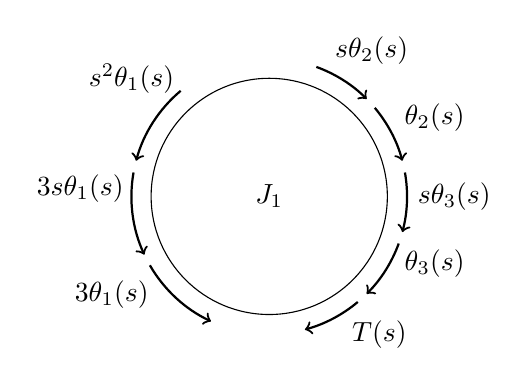
\begin{tikzpicture}
                % Circle
                \draw (0,0) circle (1.5);
                \node at (0,0) {$J_1$};
                % Left-hand Arrows
                \draw[->, thick] (0,0) ++(130:1.75) arc[start angle=130, end angle=165, radius=1.75];
                \node at (-1.75,1.5){$s^2\theta_1(s)$};
                \draw[->, thick] (0,0) ++(170:1.75) arc[start angle=170, end angle=205, radius=1.75];
                \node at (-2.4,0.1){$3s\theta_1(s)$};
                \draw[->, thick] (0,0) ++(210:1.75) arc[start angle=210, end angle=245, radius=1.75];
                \node at (-2,-1.25){$3\theta_1(s)$};
                % Right-hand Arrows
                \draw[->, thick] (0,0) ++(70:1.75) arc[start angle=70, end angle=45, radius=1.75];
                \node at (1.3,1.85){$s\theta_2(s)$};
                \draw[->, thick] (0,0) ++(40:1.75) arc[start angle=40, end angle=15, radius=1.75];
                \node at (2.1,1){$\theta_2(s)$};
                \draw[->, thick] (0,0) ++(10:1.75) arc[start angle=10, end angle=-15, radius=1.75];
                \node at (2.35,0){$s\theta_3(s)$};
                \draw[->, thick] (0,0) ++(-20:1.75) arc[start angle=-20, end angle=-45, radius=1.75];
                \node at (2.1,-0.85){$\theta_3(s)$};
                \draw[->, thick] (0,0) ++(-50:1.75) arc[start angle=-50, end angle=-75, radius=1.75];
                \node at (1.4,-1.75){$T(s)$};
            \end{tikzpicture}%
        }
                % Equations under J1

            $\sum T_0 = 0 \quad\text{(clockwise, +)}$ \\ \vspace{10pt}
            $T(s) -(s^2+3s+3)\theta_1(s) + (s+1)\theta_2(s) + (s+1)\theta_3(s) = 0$ \\ \vspace{10pt}
            $T(s) = (s^2+3s+3)\theta_1(s) - (s+1)\theta_2(s) - (s+1)\theta_3(s)$
                
        \end{center}
\newpage
	\vspace{15pt}
        \begin{center}
                \textbf{Free Body Diagram at $J_2$} \\[6pt]
                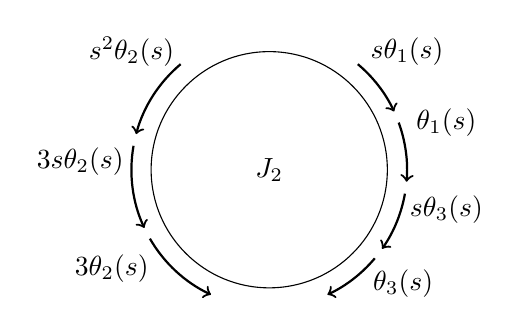
\begin{tikzpicture}
                    % Circle
                    \draw (0,0) circle (1.5);
                    \node at (0,0) {$J_2$};
                    % Left-hand Arrows
                    \draw[->, thick] (0,0) ++(130:1.75) arc[start angle=130, end angle=165, radius=1.75];
                    \node at (-1.75,1.5){$s^2\theta_2(s)$};
                    \draw[->, thick] (0,0) ++(170:1.75) arc[start angle=170, end angle=205, radius=1.75];
                    \node at (-2.4,0.1){$3s\theta_2(s)$};
                    \draw[->, thick] (0,0) ++(210:1.75) arc[start angle=210, end angle=245, radius=1.75];
                    \node at (-2,-1.25){$3\theta_2(s)$};
                    % Right-hand Arrows
                    \draw[->, thick] (0,0) ++(50:1.75) arc[start angle=50, end angle=25, radius=1.75];
                    \node at (1.75,1.5){$s\theta_1(s)$};
                    \draw[->, thick] (0,0) ++(20:1.75) arc[start angle=20, end angle=-5, radius=1.75];
                    \node at (2.25,0.6){$\theta_1(s)$};
                    \draw[->, thick] (0,0) ++(-10:1.75) arc[start angle=-10, end angle=-35, radius=1.75];
                    \node at (2.25,-0.5){$s\theta_3(s)$};
                    \draw[->, thick] (0,0) ++(-40:1.75) arc[start angle=-40, end angle=-65, radius=1.75];
                    \node at (1.7,-1.45){$\theta_3(s)$};
                \end{tikzpicture}
        
                % Equations under J2
        
        \vspace{15pt}

            $\sum T_0 = 0 \quad\text{(clockwise, +)}$ \\ \vspace{10pt}
            $0 = (s+1)\theta_1(s) - (s^2+3s+3)\theta_2(s) + (s+1)\theta_3(s)$\\ \vspace{10pt}
            $0 = -(s+1)\theta_1(s) + (s^2+3s+3)\theta_2(s) - (s+1)\theta_3(s)$

		
			\end{center}
		
    \vspace{15pt}
        	\begin{center}
                \textbf{Free Body Diagram at $J_3$} \\[6pt]
                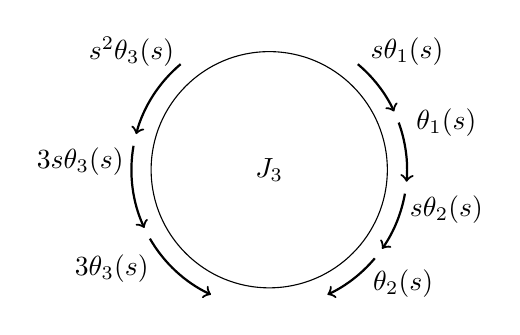
\begin{tikzpicture}
                    % Circle
                    \draw (0,0) circle (1.5);
                    \node at (0,0) {$J_3$};
                    % Left-hand Arrows
                    \draw[->, thick] (0,0) ++(130:1.75) arc[start angle=130, end angle=165, radius=1.75];
                    \node at (-1.75,1.5){$s^2\theta_3(s)$};
                    \draw[->, thick] (0,0) ++(170:1.75) arc[start angle=170, end angle=205, radius=1.75];
                    \node at (-2.4,0.1){$3s\theta_3(s)$};
                    \draw[->, thick] (0,0) ++(210:1.75) arc[start angle=210, end angle=245, radius=1.75];
                    \node at (-2,-1.25){$3\theta_3(s)$};
                    % Right-hand Arrows
                    \draw[->, thick] (0,0) ++(50:1.75) arc[start angle=50, end angle=25, radius=1.75];
                    \node at (1.75,1.5){$s\theta_1(s)$};
                    \draw[->, thick] (0,0) ++(20:1.75) arc[start angle=20, end angle=-5, radius=1.75];
                    \node at (2.25,0.6){$\theta_1(s)$};
                    \draw[->, thick] (0,0) ++(-10:1.75) arc[start angle=-10, end angle=-35, radius=1.75];
                    \node at (2.25,-0.5){$s\theta_2(s)$};
                    \draw[->, thick] (0,0) ++(-40:1.75) arc[start angle=-40, end angle=-65, radius=1.75];
                    \node at (1.7,-1.45){$\theta_2(s)$};
                \end{tikzpicture}
        
                % Equations under J2
        
        \vspace{15pt}

            $\sum T_0 = 0 \quad\text{(clockwise, +)}$ \\ \vspace{10pt}
            $0 = (s+1)\theta_1(s) + (s+1)\theta_2(s) - (s^2+3s+3)\theta_3(s)$\\ \vspace{10pt}
            $0 = -(s+1)\theta_1(s) - (s+1)\theta_2(s) + (s+1)\theta_3(s)$

		
            \end{center}
		
	\vspace{15pt}

		\item Write the displacement equations and provide the matrix form
\begin{center}
	T(s) $= (s^2 + 3s + 3)\theta_1(s) - (s + 1)\theta_2(s) - (s + 1)\theta_3(s)$\\
	0 $= -(s + 1)\theta_1(s) +(s^2 + 3s + 3)\theta_2(s) - (s + 1)\theta_3(s)$\\
	0 $= -(s + 1)\theta_1(s) - (s + 1)\theta_2(s) + (s^2 + 3s + 3)\theta_3(s)$\\
	\[
		\begin{bmatrix}
		(s^2 + 3s + 3) & -(s + 1) & -(s + 1)\\
		-(s + 1) & (s^2 + 3s + 3) & -(s + 1)\\
		-(s + 1) & -(s + 1) & (s^2 + 3s + 3)\\
		\end{bmatrix}
		\begin{bmatrix}
		\theta_1(s) \\
		\theta_2(s) \\
		\theta_3(s)
		\end{bmatrix}
		=
		\begin{bmatrix}
		T(s)\\
		0\\
		0
		\end{bmatrix}
	\]\\
\end{center}
		\item Apply Cramer's Rule to get the value of the Transfer Function
\begin{center}
	\[
		\theta_1(s) = 
			\frac{\begin{vmatrix}
				T(s) & -(s + 1) & -(s + 1)\\
				0 & (s^2 + 3s + 3) & -(s + 1)\\
				0 & -(s + 1) & (s^2 + 3s + 3)\\
			\end{vmatrix}
		}{\begin{vmatrix}
				(s^2 + 3s + 3) & -(s + 1) & -(s + 1)\\
				-(s + 1) & (s^2 + 3s + 3) & -(s + 1)\\
				-(s + 1) & -(s + 1) & (s^2 + 3s + 3)\\
			\end{vmatrix}
		}
	\]
	\[
	\theta_1(s) = \frac{(s^4 + 6s^3 + 14s^2 + 16s + 8)T(s)}{s^6 + 9s^5 + 33s^4 + 64s^3 + 72s^2 + 48s + 16}
	\] 

	\[
	\boxed{\frac{X_1(s)}{F(s)} = \frac{s^4 + 6s^3 + 14s^2 + 16s + 8}{s^6 + 9s^5 + 33s^4 + 64s^3 + 72s^2 + 48s + 16}}
	\] 

\end{center}
	\end{enumerate}


\end{fold}

% Problem 25
\begin{fold}

\newpage
\noindent\rule{\textwidth}{1pt}
\noindent\textbf{Problem 25} \hfill 
\\Given the Rotational Mechanical System below, solve for the Transfer Function $\frac{\theta_1(s)}{F(s)}$\\

\begin{center}
	\begin{tikzpicture}[scale = 0.68, every node/.append style={font=\scriptsize}]
		% wall
            
		\def\brickw{0.24}   % brick width
		\def\brickh{0.18} % brick height
		\def\nrows{64}   % number of rows
		% draw bricks row by row
        \begin{scope}[shift={(-4,0)}]
		\foreach \r in {0,...,\nrows} {
			% shift every other row
			\pgfmathparse{mod(\r,2)==0 ? 0 : 0.5*\brickw}
			\let\shift\pgfmathresult
			\foreach \c in {0,1} {
			\draw[thick] (\shift+\c*\brickw, \r*\brickh) rectangle ++(\brickw,\brickh);
		}}
		\draw (0,0) rectangle (0.6,11.7);
        
            \end{scope}
        \begin{scope}[shift={(-1.5,0)}]
    		% spring
    		\draw (-1.9,1.25) [cute inductor=] to (2,1.25);
    		% mass damper
    		\draw (-1.9,3.75) to (-0.2,3.75);
                \begin{scope}[shift={(-1,2.35)}]
    		\draw (0.8,1) to (0.8, 1.8);
    		\draw (0.8,1) to (1.6, 1);
    		\draw (0.8,1.8) to (1.6, 1.8);
    		\draw (1.2, 1.2) to (1.2, 1.6);
                \end{scope}
    		\draw (0.2,3.75) to (2, 3.75);
        \end{scope}
		\begin{scope}[shift={(-1,0)}]
			%Inertia 1
			\draw (1.5,5.5) -- (4.1,5.5);
			\draw (1.5,-0.5) -- (4.1,-0.5);
			\draw (1.5,2.5) ellipse (0.15 and 3);
			\draw (4.1,-0.5) arc[start angle=-90, end angle=90, x radius=0.2, y radius=3];
		\end{scope}	
        \begin{scope}[shift={(-0.5,2.25)}]
		% spring
    		\draw (3.8,0.65) [cute inductor=] to (6.7,0.65);
    		% mass damper
    		\draw (3.75,2) to (4.75,2);
                \begin{scope}[shift={(-0.25,0.6)}]
    		\draw (5,1) to (5, 1.8);
    		\draw (5,1) to (5.8, 1);
    		\draw (5,1.8) to (5.8, 1.8);
    		\draw (5.4, 1.2) to (5.4, 1.6);
                \end{scope}
    		\draw (5.15,2) to (6.7, 2);
			\begin{scope}[shift={(0.5,0)}]
				%Inertia 2
				\draw (6.2,6) -- (8.8,6);
				\draw (6.2,0) -- (8.8,0);
				\draw (6.2,3) ellipse (0.2 and 3);
				\draw (8.8,0) arc[start angle=-90, end angle=90, x radius=0.275, y radius=3];
        	\end{scope}
		\end{scope}

			\begin{scope}[shift={(0,2.55)}]
                % spring
                \draw (9.05,1.65) [cute inductor=] to (12.4,1.65);
            	% mass damper
            	\draw (9.05,4.4) to (10.2,4.4);
                    \begin{scope}[shift={(1,2)}]
            	\draw (9.2,2) to (9.2, 2.8);
            	\draw (9.2,2) to (10, 2);
            	\draw (9.2,2.8) to (10, 2.8);
            	\draw (9.6, 2.2) to (9.6, 2.6);
                    \end{scope}
            	\draw (10.6,4.4) to (12.4, 4.4);
            \end{scope}
        
        \begin{scope}[shift={(-1,3.5)}]
            % long damper and spring
            \draw (-2.35,2.75) [cute inductor=] to (7.2,2.75);
    		% mass damper
    		\draw (-2.35,4.25) to (2.05,4.25);
                \begin{scope}[shift={(-1,0.5)}]
    		\draw (3.05,3.35) to (3.05, 4.15);
    		\draw (3.05,3.35) to (3.85, 3.35);
    		\draw (3.05,4.15) to (3.85, 4.15);
    		\draw (3.45, 3.55) to (3.45, 3.95);
                \end{scope}
    		\draw (2.45,4.25) to (7.2, 4.25);
        \end{scope}
        %Inertia 3
  		\draw (12.4,11) -- (15,11);
  		\draw (12.4,-0.5) -- (15,-0.5);
  		\draw (12.4,5.25) ellipse (0.2 and 5.75);
  		\draw (15,-0.5) arc[start angle=-90, end angle=90, x radius=0.275, y radius=5.75];
        \begin{scope}[shift={(5,-2.5)}]
            % long damper and spring
            \draw (-1.775,2.25) [cute inductor=] to (7.4,2.25);
    		% mass damper
    		\draw (-1.725,3.75) to (2.25,3.75);
                \begin{scope}[shift={(-0.8,0)}]
    		\draw (3.05,3.35) to (3.05, 4.15);
    		\draw (3.05,3.35) to (3.85, 3.35);
    		\draw (3.05,4.15) to (3.85, 4.15);
    		\draw (3.45, 3.55) to (3.45, 3.95);
                \end{scope}
    		\draw (2.65,3.75) to (7.4, 3.75);
        \end{scope}
        \begin{scope}[shift={(6.2,2.75)}]
            % spring
            \draw (9.05,0) [cute inductor=] to (12.4,0);
        	% mass damper
        	\draw (9.05,4.4) to (10.2,4.4);
                \begin{scope}[shift={(1,2)}]
        	\draw (9.2,2) to (9.2, 2.8);
        	\draw (9.2,2) to (10, 2);
        	\draw (9.2,2.8) to (10, 2.8);
        	\draw (9.6, 2.2) to (9.6, 2.6);
                \end{scope}
        	\draw (10.6,4.4) to (12.4, 4.4);
        \end{scope}
        \begin{scope}[shift={(-1,7)}]
            % long damper and spring
            \draw (-2.4,2.25) [cute inductor=] to (13.35,2.25);
    		% mass damper
    		\draw (-2.4,3.75) to (5.05,3.75);
                \begin{scope}[shift={(2,0)}]
    		\draw (3.05,3.35) to (3.05, 4.15);
    		\draw (3.05,3.35) to (3.85, 3.35);
    		\draw (3.05,4.15) to (3.85, 4.15);
    		\draw (3.45, 3.55) to (3.45, 3.95);
                \end{scope}
    		\draw (5.45,3.75) to (13.35, 3.75);
        \end{scope}
		% wall
		\def\brickw{0.24}   % brick width
		\def\brickh{0.18} % brick height
		\def\nrows{64}   % number of rows
		% draw bricks row by row
		\begin{scope}[shift={(18.62,0)}]
			\foreach \r in {0,...,\nrows} {
				% shift every other row
				\pgfmathparse{mod(\r,2)==0 ? 0 : 0.5*\brickw}
				\let\shift\pgfmathresult
				\foreach \c in {0,1} {
				\draw[thick] (\shift+\c*\brickw, \r*\brickh) rectangle ++(\brickw,\brickh);
			}}
			\draw (0,0) rectangle (0.61,11.7);
		\end{scope}
		
		% Label 1
		\node[scale=0.70] at (-1.4, 0.6) {$6N-m/rad$};
        \node[scale=0.70] at (-1.5, 2.9) {$3N\cdot m\cdot s/rad$};
		\node[scale=0.70] at (2, 2.5) {$1kg\cdot m^2$};
        \node[scale=0.70] at (4.6, 3.5) {$7N-m/rad$};
        \node[scale=0.70] at (4.6, 5) {$4N\cdot m\cdot s/rad$};
        % Label 2
		\node[scale=0.70] at (7.65, 0.5) {$6N-m-s/rad$};
		\node[scale=0.70] at (7.75, -0.9) {$3N-m/rad$};
		\node[scale=0.70] at (7.65, 5.25) {$1kg-m^2$};
        \begin{scope}[shift={(0,2.6)}]
            \node[scale=0.70] at (10.6, 3.65) {$3N\cdot m\cdot s/rad$};
    		\node[scale=0.70] at (10.5, 1.05) {$4N-m/rad$};
    	\end{scope}
       	\begin{scope}[shift={(-9,5.65)}]
           \node[scale=0.70] at (10.5, 3) {$3N-m-s/rad$};
    		\node[scale=0.70] at (10.5, 1.25) {$4N-m/rad$};
	   	\end{scope}
    	%Label 3
        \begin{scope}[shift={(6.2,2.75)}]
           	\node[scale=0.70] at (10.6, 5.25) {$3N\cdot m\cdot s/rad$};
    		\node[scale=0.70] at (10.5, 0.7) {$3N-m/rad$};
        \end{scope}
       	\begin{scope}[shift={(-6,8.65)}]
           	\node[scale=0.70] at (10.5, 3) {$5N-m-s/rad$};
    		\node[scale=0.70] at (10.5, 1.25) {$11N-m/rad$};
       	\end{scope}
       	\node[scale=0.70] at (14,5) {$1kg-m^2$};

		% Arrows 1
		\draw[<-,cyan] (1.75,5.5) arc[start angle=60,end angle=300,x radius=0.5,y radius=3.55];
		\node[cyan, scale=0.70] at (2.5,-1.65) {$\theta_1(t)$};
		\draw[<-,cyan] (2.5,5.5) arc[start angle=60,end angle=300,x radius=0.5,y radius=3.55];
		\node[cyan, scale=0.70] at (1.5,-1.65) {$T(t)$};
		% Arrows 2
		\begin{scope}[shift={(6.25,2.75)}]
           	\draw[<-,cyan] (1.85,5.6) arc[start angle=60,end angle=300,x radius=0.5,y radius=3.55];
			\node[cyan, scale=0.70] at (2.5,6) {$\theta_2(t)$};
       	\end{scope}
        % Arrows 3
        \begin{scope}[shift={(12.5,4.6)}]
           	\draw[<-,cyan] (1.85,6.5) arc[start angle=60,end angle=300,x radius=0.5,y radius=6.8];
			\node[cyan, scale=0.70] at (2.5,7) {$\theta_3(t)$};
        \end{scope}
	\end{tikzpicture}
\end{center}

\noindent\rule{\textwidth}{1pt}\\

\noindent \textbf{\textit{Given:}}\\

\[
\begin{aligned}
J_1 &= 1\,\text{kg·m}^2 \qquad & f_{v1} &= 3\,\text{N·m·s/rad} \qquad & K_1 &= 6\,\text{N·m/rad} \\
J_2 &= 1\,\text{kg·m}^2 \qquad & f_{v2} &= 6\,\text{N·m·s/rad} \qquad & K_2 &= 3\,\text{N·m/rad} \\
J_3 &= 1\,\text{kg·m}^2 \qquad & f_{v3} &= 4\,\text{N·m·s/rad} \qquad & K_3 &= 7\,\text{N·m/rad} \\
&& f_{v4} &= 5\,\text{N·m·s/rad} \qquad & K_4 &= 4\,\text{N·m/rad} \\
&& f_{v5} &= 3\,\text{N·m·s/rad} \qquad & K_5 &= 4\,\text{N·m/rad} \\
&& f_{v6} &= 3\,\text{N·m·s/rad} \qquad & K_6 &= 3\,\text{N·m/rad} \\
&& f_{v7} &= 5\,\text{N·m·s/rad} \qquad & K_7 &= 11\,\text{N·m/rad}
\end{aligned}
\]


\noindent \textbf{\textit{Required:}}\\

\begin{center}
	$\dfrac{\theta_1(s)}{T(s)}$
\end{center}

	\noindent \textbf{\textit{Solution:}}\\

% Start of Solution
\begin{enumerate}[label=(\alph*),itemindent=*,leftmargin=*,nolistsep]
\item Draw the Free Body Diagrams of the provided masses
\vspace{15pt}

%---------------- J1 ----------------%
\begin{center}
\textbf{Free Body Diagram at $J_1$} \\[6pt]
\scalebox{0.60}{%
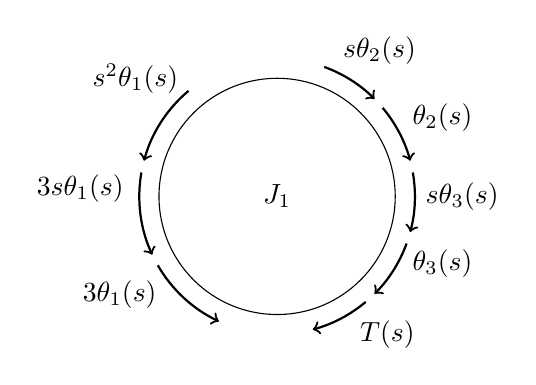
\begin{tikzpicture}
    \draw (0,0) circle (1.5);
    \node at (0,0) {$J_1$};
    % Left-hand Arrows
    \draw[->, thick] (0,0) ++(130:1.75) arc[start angle=130, end angle=165, radius=1.75];
    \node at (-1.8,1.5){$s^2\theta_1(s)$};
    \draw[->, thick] (0,0) ++(170:1.75) arc[start angle=170, end angle=205, radius=1.75];
    \node at (-2.5,0.1){$3s\theta_1(s)$};
    \draw[->, thick] (0,0) ++(210:1.75) arc[start angle=210, end angle=245, radius=1.75];
    \node at (-2,-1.25){$3\theta_1(s)$};
    % Right-hand Arrows
    \draw[->, thick] (0,0) ++(70:1.75) arc[start angle=70, end angle=45, radius=1.75];
    \node at (1.3,1.85){$s\theta_2(s)$};
    \draw[->, thick] (0,0) ++(40:1.75) arc[start angle=40, end angle=15, radius=1.75];
    \node at (2.1,1){$\theta_2(s)$};
    \draw[->, thick] (0,0) ++(10:1.75) arc[start angle=10, end angle=-15, radius=1.75];
    \node at (2.35,0){$s\theta_3(s)$};
    \draw[->, thick] (0,0) ++(-20:1.75) arc[start angle=-20, end angle=-45, radius=1.75];
    \node at (2.1,-0.85){$\theta_3(s)$};
    \draw[->, thick] (0,0) ++(-50:1.75) arc[start angle=-50, end angle=-75, radius=1.75];
    \node at (1.4,-1.75){$T(s)$};
\end{tikzpicture}
}
\vspace{10pt}

$\sum T_0 = 0 \quad\text{(clockwise, +)}$ \\[6pt]
$T(s) -(5s^2+7s+13)\theta_1(s) + (4s+7)\theta_2(s) + (6s+3)\theta_3(s) = 0$ \\[6pt]
$T(s) = (5s^2+7s+13)\theta_1(s) - (4s+7)\theta_2(s) - (6s+3)\theta_3(s)$
\end{center}

%---------------- J2 ----------------%
\begin{center}
\textbf{Free Body Diagram at $J_2$} \\[6pt]
\scalebox{0.60}{%
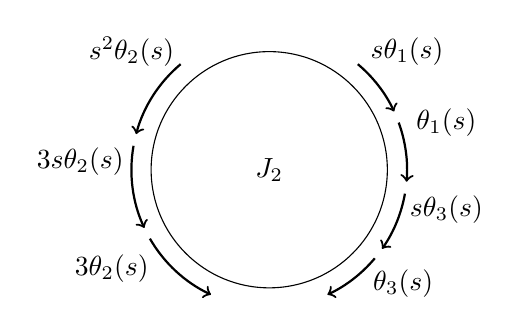
\begin{tikzpicture}
    \draw (0,0) circle (1.5);
    \node at (0,0) {$J_2$};
    % Left-hand Arrows
    \draw[->, thick] (0,0) ++(130:1.75) arc[start angle=130, end angle=165, radius=1.75];
    \node at (-1.75,1.5){$s^2\theta_2(s)$};
    \draw[->, thick] (0,0) ++(170:1.75) arc[start angle=170, end angle=205, radius=1.75];
    \node at (-2.4,0.1){$3s\theta_2(s)$};
    \draw[->, thick] (0,0) ++(210:1.75) arc[start angle=210, end angle=245, radius=1.75];
    \node at (-2,-1.25){$3\theta_2(s)$};
    % Right-hand Arrows
    \draw[->, thick] (0,0) ++(50:1.75) arc[start angle=50, end angle=25, radius=1.75];
    \node at (1.75,1.5){$s\theta_1(s)$};
    \draw[->, thick] (0,0) ++(20:1.75) arc[start angle=20, end angle=-5, radius=1.75];
    \node at (2.25,0.6){$\theta_1(s)$};
    \draw[->, thick] (0,0) ++(-10:1.75) arc[start angle=-10, end angle=-35, radius=1.75];
    \node at (2.25,-0.5){$s\theta_3(s)$};
    \draw[->, thick] (0,0) ++(-40:1.75) arc[start angle=-40, end angle=-65, radius=1.75];
    \node at (1.7,-1.45){$\theta_3(s)$};
\end{tikzpicture}
}
\vspace{10pt}

$\sum T_0 = 0 \quad\text{(clockwise, +)}$ \\[6pt]
$0 = (4s+7)\theta_1(s) - (7s^2+9s+11)\theta_2(s) + (5s+4)\theta_3(s)$ \\[6pt]
$0 = -(4s+7)\theta_1(s) + (7s^2+9s+11)\theta_2(s) - (5s+4)\theta_3(s)$
\end{center}

%---------------- J3 ----------------%
\begin{center}
\textbf{Free Body Diagram at $J_3$} \\[6pt]
\scalebox{0.60}{%
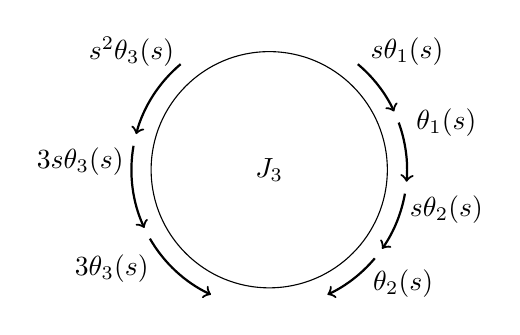
\begin{tikzpicture}
    \draw (0,0) circle (1.5);
    \node at (0,0) {$J_3$};
    % Left-hand Arrows
    \draw[->, thick] (0,0) ++(130:1.75) arc[start angle=130, end angle=165, radius=1.75];
    \node at (-1.75,1.5){$s^2\theta_3(s)$};
    \draw[->, thick] (0,0) ++(170:1.75) arc[start angle=170, end angle=205, radius=1.75];
    \node at (-2.4,0.1){$3s\theta_3(s)$};
    \draw[->, thick] (0,0) ++(210:1.75) arc[start angle=210, end angle=245, radius=1.75];
    \node at (-2,-1.25){$3\theta_3(s)$};
    % Right-hand Arrows
    \draw[->, thick] (0,0) ++(50:1.75) arc[start angle=50, end angle=25, radius=1.75];
    \node at (1.75,1.5){$s\theta_1(s)$};
    \draw[->, thick] (0,0) ++(20:1.75) arc[start angle=20, end angle=-5, radius=1.75];
    \node at (2.25,0.6){$\theta_1(s)$};
    \draw[->, thick] (0,0) ++(-10:1.75) arc[start angle=-10, end angle=-35, radius=1.75];
    \node at (2.25,-0.5){$s\theta_2(s)$};
    \draw[->, thick] (0,0) ++(-40:1.75) arc[start angle=-40, end angle=-65, radius=1.75];
    \node at (1.7,-1.45){$\theta_2(s)$};
\end{tikzpicture}
}
\vspace{10pt}

$\sum T_0 = 0 \quad\text{(clockwise, +)}$ \\[6pt]
$0 = (6s+3)\theta_1(s) + (5s+4)\theta_2(s) - (s^2+19s+21)\theta_3(s)$ \\[6pt]
$0 = -(6s+3)\theta_1(s) - (5s+4)\theta_2(s) + (s^2+19s+21)\theta_3(s)$
\end{center}

\vspace{15pt}
\item Write the displacement equations and provide the matrix form
\begin{center}
T(s) $= (5s^2 + 7s + 13)\theta_1(s) - (4s + 7)\theta_2(s) - (6s + 3)\theta_3(s)$\\
0 $= -(4s + 7)\theta_1(s) +(7s^2 + 9s + 11)\theta_2(s) - (5s + 4)\theta_3(s)$\\
0 $= -(6s + 3)\theta_1(s) - (5s + 4)\theta_2(s) + (s^2 + 19s + 21)\theta_3(s)$\\
\[
\begin{bmatrix}
(5s^2 + 7s + 13) & -(4s + 7) & -(6s + 3)\\
-(4s + 7) & (7s^2 + 9s + 11) & -(5s + 4)\\
-(6s + 3) & -(5s + 4) & (s^2 + 19s + 21)\\
\end{bmatrix}
\begin{bmatrix}
\theta_1(s) \\
\theta_2(s) \\
\theta_3(s)
\end{bmatrix}
=
\begin{bmatrix}
T(s)\\
0\\
0
\end{bmatrix}
\]
\end{center}

\end{enumerate}


\vspace{15pt}
\item Write the displacement equations and provide the matrix form
\begin{center}
T(s) $= (5s^2 + 7s + 13)\theta_1(s) - (4s + 7)\theta_2(s) - (6s + 3)\theta_3(s)$\\
0 $= -(4s + 7)\theta_1(s) +(7s^2 + 9s + 11)\theta_2(s) - (5s + 4)\theta_3(s)$\\
0 $= -(6s + 3)\theta_1(s) - (5s + 4)\theta_2(s) + (s^2 + 19s + 21)\theta_3(s)$\\
\[
\begin{bmatrix}
(5s^2 + 7s + 13) & -(4s + 7) & -(6s + 3)\\
-(4s + 7) & (7s^2 + 9s + 11) & -(5s + 4)\\
-(6s + 3) & -(5s + 4) & (s^2 + 19s + 21)\\
\end{bmatrix}
\begin{bmatrix}
\theta_1(s) \\
\theta_2(s) \\
\theta_3(s)
\end{bmatrix}
=
\begin{bmatrix}
T(s)\\
0\\
0
\end{bmatrix}
\]
\end{center}

		\item Apply Cramer's Rule to get the value of the Transfer Function
\begin{center}
	\[
		\theta_1(s) = 
			\frac{\begin{vmatrix}
				T(s) & -(4s + 7) & -(6s + 3)\\
				0 & (7s^2 + 9s + 11)  & -(5s + 4)\\
				0 & -(5s + 4) & (s^2 + 19s + 21)\\
			\end{vmatrix}
		}{\begin{vmatrix}
				(5s^2 + 7s + 13) & -(4s + 7) & -(6s + 3)\\
				-(4s + 7) & (7s^2 + 9s + 11) & -(5s + 4)\\
				-(6s + 3) & -(5s + 4) & (s^2 + 19s + 21)\\
			\end{vmatrix}
		}
	\]
	\[
	\theta_1(s) = \frac{(7s^4 + 142s^3 + 304s^2 + 358s + 215)T(s)}{35s^6 + 759s^5 + 2337s^4 + 4588s^3 + 4569s^2 + 2933s + 1499}
	\] 

	\[
	\boxed{\frac{X_1(s)}{F(s)} = \frac{7s^4 + 142s^3 + 304s^2 + 358s + 215}{35s^6 + 759s^5 + 2337s^4 + 4588s^3 + 4569s^2 + 2933s + 1499}}
	\] 

\end{center}


\end{fold}